% !TEX program = xelatex
% =============================================================================
% Block Round --- Plano de Aula (pt-BR)
% Sequencia didatica de 5 aulas para o 3.o ano do Ensino Medio (escola publica
% brasileira), ancorada no universo Minecraft.
% Estilo grafico alinhado a docs_math/Block_Round_Math_pt-BR.pdf
% Compilacao: xelatex Plano_de_Aula_pt-BR.tex  (executar duas vezes p/ TOC + refs)
% =============================================================================
\documentclass[12pt,a4paper]{scrartcl}

% ---------- Idioma e fontes (identico ao docs_math) --------------------------
\usepackage{fontspec}
\usepackage{polyglossia}
\setdefaultlanguage{portuguese}
\PolyglossiaSetup{portuguese}{indentfirst=false}
\setmainfont{Latin Modern Roman}[Scale=1.08]
\setsansfont{Latin Modern Sans}[Scale=1.08]
\setmonofont{Latin Modern Mono}[Scale=1.00]
\usepackage{unicode-math}
\setmathfont{Latin Modern Math}[Scale=1.08]

% ---------- Pacotes ----------------------------------------------------------
\usepackage{amsmath}
\usepackage{mathtools}

\usepackage[a4paper,top=2.8cm,bottom=2.8cm,left=2.6cm,right=2.6cm,
            headheight=16pt]{geometry}
\usepackage{microtype}
\usepackage{xcolor}
\usepackage{booktabs}
\usepackage{array}
\usepackage{tabularx}
\usepackage{enumitem}
\usepackage{titlesec}
\usepackage{fancyhdr}
\usepackage{graphicx}
\usepackage{csquotes}
\usepackage{tcolorbox}
\tcbuselibrary{skins,breakable}
\usepackage{needspace}
\usepackage{caption}
\usepackage{subcaption}
\usepackage{float}

\raggedbottom

% ---------- Paleta cromatica Block Round -------------------------------------
\definecolor{accent}{HTML}{5B8E3F}      % verde-grama Minecraft
\definecolor{accentdark}{HTML}{406A2A}
\definecolor{earth}{HTML}{825432}        % marrom-dirt
\definecolor{ink}{HTML}{1F1F23}
\definecolor{muted}{HTML}{4E4E58}
\definecolor{bg}{HTML}{FBF6E9}
\definecolor{rule}{HTML}{D8D1BC}
\definecolor{linkc}{HTML}{2D5A1F}        % verde mais escuro p/ links

\usepackage[colorlinks=true,
            linkcolor=linkc,
            urlcolor=linkc,
            citecolor=linkc,
            breaklinks=true,
            bookmarks=true,bookmarksopen=true,
            pdftitle={Block Round --- Plano de Aula (pt-BR)},
            pdfauthor={Vinicius Rodrigues de Souza}]{hyperref}
% xurl permite quebrar URLs em qualquer caractere (alternativa: url
% so quebra em pontos pre-definidos). Carregado DEPOIS de hyperref.
\usepackage{xurl}

\color{ink}

\widowpenalty=10000
\clubpenalty=10000

% ---------- Estilo de secoes -------------------------------------------------
\titleformat{\section}
  {\sffamily\Large\bfseries\color{accent}}{\thesection.}{0.6em}{}
\titleformat{\subsection}
  {\sffamily\large\bfseries\color{accent!85!ink}}{\thesubsection}{0.6em}{}
\titleformat{\subsubsection}
  {\sffamily\normalsize\bfseries\color{muted}}{\thesubsubsection}{0.5em}{}
\titlespacing*{\section}{0pt}{1.2\baselineskip}{0.6\baselineskip}
\titlespacing*{\subsection}{0pt}{0.8\baselineskip}{0.3\baselineskip}
\titlespacing*{\subsubsection}{0pt}{0.6\baselineskip}{0.2\baselineskip}

% ---------- Cabecalho e rodape -----------------------------------------------
\pagestyle{fancy}
\fancyhf{}
\fancyhead[L]{\small\sffamily\bfseries\color{accent}BLOCK ROUND}
\fancyhead[R]{\small\sffamily\color{muted}Plano de Aula --- 3.\textordmasculine\ ano EM}
\fancyfoot[L]{\small\sffamily\color{muted}Block Round --- Material didatico}
\fancyfoot[R]{\small\sffamily\color{muted}Pagina \thepage}
\renewcommand{\headrulewidth}{0.4pt}
\renewcommand{\footrulewidth}{0.4pt}
\renewcommand{\headrule}{{\color{rule}\hrule height \headrulewidth}}
\renewcommand{\footrule}{{\color{rule}\vskip-\footrulewidth\hrule height \footrulewidth\vskip-\footrulewidth}}

% ---------- Caixas didaticas -------------------------------------------------
\newtcolorbox{formula}{
  colback=bg, colframe=rule, boxrule=0.4pt, arc=2pt,
  left=10pt,right=10pt,top=8pt,bottom=8pt,
  before skip=8pt, after skip=8pt,
  fontupper=\color{accentdark}, breakable,
  before={\par\needspace{4\baselineskip}}
}

\newtcolorbox{atividade}[1][Atividade]{
  enhanced, breakable,
  colback=bg, colframe=accent, boxrule=0.6pt, arc=4pt,
  left=12pt,right=12pt,top=10pt,bottom=10pt,
  before skip=12pt, after skip=12pt,
  before={\par\needspace{5\baselineskip}},
  attach boxed title to top left={xshift=10pt,yshift=-8pt},
  boxed title style={colback=accent,colframe=accent,boxrule=0pt,arc=2pt},
  coltitle=white, fonttitle=\sffamily\bfseries\small,
  title=#1
}

\newtcolorbox{nota}[1][Nota didatica]{
  enhanced, breakable,
  colback=bg!50!white, colframe=rule, boxrule=0.4pt, arc=2pt,
  left=10pt,right=10pt,top=8pt,bottom=8pt,
  before skip=8pt, after skip=8pt,
  before={\par\needspace{3\baselineskip}},
  attach boxed title to top left={xshift=10pt,yshift=-7pt},
  boxed title style={colback=muted,colframe=muted,boxrule=0pt,arc=2pt},
  coltitle=white, fonttitle=\sffamily\bfseries\footnotesize,
  title=#1
}

\newtcolorbox{habilidade}[1][BNCC]{
  enhanced,
  breakable=false,
  colback=bg!70!white, colframe=accent!60!ink, boxrule=0.4pt, arc=2pt,
  left=10pt,right=10pt,top=6pt,bottom=6pt,
  before skip=6pt, after skip=6pt,
  before={\par\needspace{8\baselineskip}},
  attach boxed title to top left={xshift=10pt,yshift=-6pt},
  boxed title style={colback=accent!60!ink,colframe=accent!60!ink,boxrule=0pt,arc=2pt},
  coltitle=white, fonttitle=\sffamily\bfseries\footnotesize,
  title=#1
}

\newtcolorbox{minec}[1][Minecraft]{
  enhanced, breakable,
  colback=accent!7, colframe=earth!70!accent, boxrule=0.5pt, arc=3pt,
  left=10pt,right=10pt,top=8pt,bottom=8pt,
  before skip=10pt, after skip=10pt,
  before={\par\needspace{3\baselineskip}},
  attach boxed title to top left={xshift=10pt,yshift=-7pt},
  boxed title style={colback=earth,colframe=earth,boxrule=0pt,arc=2pt},
  coltitle=white, fonttitle=\sffamily\bfseries\footnotesize,
  title=#1
}

\setlength{\parskip}{0.75em}
\setlength{\parindent}{0pt}
\linespread{1.10}

\setlength{\textfloatsep}{14pt plus 2pt minus 2pt}
\setlength{\floatsep}{14pt plus 2pt minus 2pt}
\setlength{\intextsep}{14pt plus 2pt minus 2pt}

\captionsetup{font=small, labelfont={bf,color=accent}, textfont={color=muted}, justification=centering}
\captionsetup[sub]{font=footnotesize, labelfont={bf,color=accent!75!ink}, textfont={color=muted}}

\graphicspath{{img/}}

\newcommand{\code}[1]{\texttt{\small #1}}
\newcommand{\acc}[1]{\textcolor{accent}{\textbf{#1}}}
\newcommand{\cmd}[1]{\textcolor{earth}{\texttt{\small #1}}}
\newcommand{\tempo}[1]{\textnormal{\footnotesize\color{bg!90!white}\textsf{#1}}}

\begin{document}

% =============================================================================
% CAPA
% =============================================================================
\begin{titlepage}
  \centering
  \vspace*{3.0cm}
  {\sffamily\bfseries\fontsize{56}{60}\selectfont \color{accent} Block Round\par}
  \vspace{0.7cm}
  {\sffamily\LARGE\color{muted} Plano de Aula\par}
  \vspace{0.25cm}
  {\sffamily\Large\color{muted} 3.\textordmasculine\ ano do Ensino Medio\par}
  \vspace{1.0cm}
  {\color{rule}\rule{0.6\textwidth}{0.6pt}\par}
  \vspace{0.7cm}
  \begin{minipage}{0.84\textwidth}
    \centering\color{ink}\large
    Sequencia didatica de cinco aulas para apresentar o gerador
    \emph{Block Round} a turmas do Ensino Medio da rede publica
    brasileira. Articula \emph{geometria analitica}, \emph{pensamento
    computacional}, \emph{cultura digital} e \emph{construcao no jogo
    Minecraft} em torno de um unico problema: como representar uma
    curva continua sobre uma malha finita de voxels, e como traduzir
    essa representacao em uma estrutura constru\'\i vel dentro do
    universo cultural mais popular entre adolescentes brasileiros.
  \end{minipage}
  \vspace{0.7cm}\\
  {\color{rule}\rule{0.6\textwidth}{0.6pt}\par}
  \vspace{0.9cm}
  \begin{minipage}{0.78\textwidth}
    \centering
    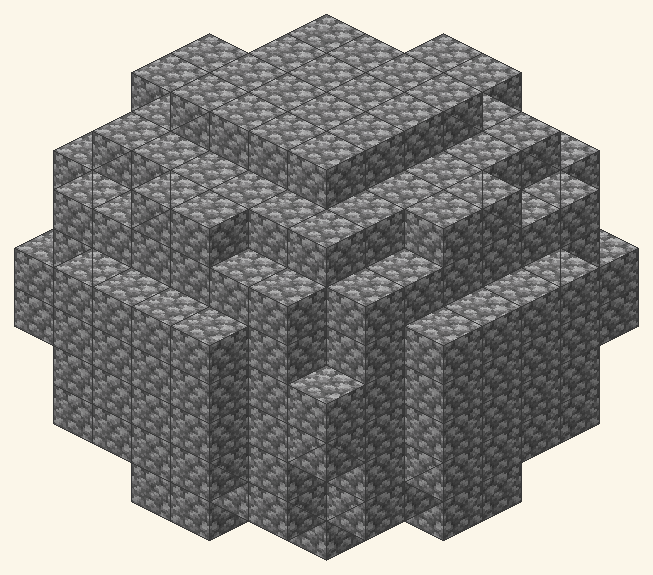
\includegraphics[width=0.55\linewidth]{fig10_3d_sphere_d12.png}\\[0.4em]
    {\sffamily\footnotesize\color{muted}Esfera de diametro 10 voxelizada pelo Block Round, renderizada com a textura \emph{cobblestone} (pedregulho) do Minecraft.}
  \end{minipage}
  \vspace{0.7cm}\\
  {\color{rule}\rule{0.6\textwidth}{0.6pt}\par}
  \vspace{0.9cm}
  \begin{minipage}{0.82\textwidth}
    \centering\sffamily\small\color{muted}
    \textbf{Areas integradas:} Matematica $\cdot$ Linguagens (Arte digital, design) $\cdot$ Computacao $\cdot$ Cultura Digital $\cdot$ Educacao para o jogo \\[0.4em]
    \textbf{Alinhamento:} BNCC --- Ensino Medio $\cdot$ Novo Ensino Medio (Lei 14.945/2024) $\cdot$ ENEM $\cdot$ \hyperref[sec:obmep]{OBMEP} $\cdot$ Minecraft Education
  \end{minipage}
\end{titlepage}

% =============================================================================
\renewcommand{\contentsname}{\color{accent}Sumario}
\tableofcontents
\thispagestyle{fancy}
\newpage

% =============================================================================
\section{Identificacao e contextualizacao}\label{sec:identificacao}

\begin{center}
\begin{tabular}{@{}p{0.32\textwidth}p{0.62\textwidth}@{}}
\toprule
\textbf{Componente curricular} & Matematica (com forte articulacao interdisciplinar: Arte, Computacao, Engenharia, Historia, Geografia). \\
\addlinespace[2pt]
\textbf{Etapa e ano} & Ensino Medio --- 3.\textordmasculine\ ano. Adaptavel para 2.\textordmasculine\ ano e para a Educacao de Jovens e Adultos (EJA). \\
\addlinespace[2pt]
\textbf{Modalidades atendidas} & Regular diurno, regular noturno, EJA, ensino integral, ensino tecnico (cursos integrados ao EM nos Institutos Federais e CEFETs). \\
\addlinespace[2pt]
\textbf{Carga horaria} & 5 aulas de 50 minutos (250 min em sala) + atividades extraclasse opcionais. Variante de 2 aulas geminadas de 100 min descrita em §\ref{sec:adapt}. \\
\addlinespace[2pt]
\textbf{Recurso central} & Block Round --- aplicacao \emph{web} gratuita, sem cadastro, sem servidor, executa offline no navegador (PWA). Conforme a LGPD: nao coleta nem transmite dados pessoais. Roda em \emph{smartphone} de baixo custo --- nao exige Java, nao exige instalar Minecraft. \\
\addlinespace[2pt]
\textbf{Eixos BNCC} & Geometria e Medidas $\cdot$ Numeros e Algebra $\cdot$ TCT \emph{Cultura Digital} (Tema Contemporaneo Transversal). \\
\addlinespace[2pt]
\textbf{Itinerarios formativos (NEM)} & \emph{Matematica e suas Tecnologias} (principal); \emph{Linguagens e suas Tecnologias} (arte digital, narrativa em jogos); \emph{Ciencias Humanas e Sociais Aplicadas} (cultura digital, midias sociais). Adequado a unidades curriculares de Aprofundamento, a projetos de Vida e a Iniciacao Cientifica. \\
\addlinespace[2pt]
\textbf{Articulacoes} & \hyperref[sec:obmep]{OBMEP} (Olimpiada Brasileira de Matematica das Escolas Publicas) $\cdot$ OBI (Olimpiada Brasileira de Informatica) $\cdot$ Feiras de Ciencias $\cdot$ Minecraft Education Edition (MEC--Microsoft). \\
\addlinespace[2pt]
\textbf{Conhecimentos previos do aluno} & Plano cartesiano; equacao da circunferencia (1.\textordmasculine\ ano); area e volume de figuras elementares (2.\textordmasculine\ ano); nocao de funcao; proporcao e porcentagem. Familiaridade com \emph{Minecraft} (recomendavel mas nao obrigatoria; o software \emph{Block Round} dispensa-a). \\
\addlinespace[2pt]
\textbf{Preparo do professor} & 20 minutos de exploracao previa do Block Round; leitura de \texttt{docs\_math/Block\_Round\_Math\_pt-BR.pdf} (documento tecnico em portugues); opcionalmente, contato superficial com os comandos \cmd{/fill}, \cmd{/clone} e \cmd{//sphere} do Minecraft Java Edition. \\
\bottomrule
\end{tabular}
\end{center}

\begin{nota}[Diversidade da escola publica brasileira]
Esta sequencia foi pensada para o contexto plural do Ensino Medio publico brasileiro: a escola estadual urbana de Sao Paulo, Recife ou Manaus; o Instituto Federal num municipio do interior; o CEFET; a escola do campo em assentamento de reforma agraria; a escola indigena em terra demarcada; a escola quilombola; a EJA no turno noturno; os programas Pe-de-Meia e Foi-de-Meia (Lei 14.818/2024). Cada um desses contextos pede ajustes especificos, mapeados em §\ref{sec:adapt}. O Block Round foi escolhido porque \emph{atende todos eles}: roda em \emph{smartphone} de baixo custo, dispensa internet apos a primeira carga (PWA), nao exige cadastro nem CPF, e nao coleta dados pessoais --- condicao exigida pela LGPD.
\end{nota}

\begin{minec}[Por que ancorar a sequencia em Minecraft]
Minecraft e o videogame mais vendido da historia (mais de 300 milhoes de copias). No Brasil, e referencia cultural transversal entre adolescentes de todas as regioes e classes sociais, atravessando barreiras de renda que outros videogames nao conseguem (a versao Pocket Edition para celular custa em torno de R\$25, e existe \emph{Minecraft Education Edition} gratuito para escolas via parceria MEC--Microsoft). Em pesquisa do \emph{Centro Regional de Estudos para o Desenvolvimento da Sociedade da Informacao} (Cetic.br/CGI.br) sobre uso de TIC entre jovens, Minecraft figura recorrentemente entre os tres jogos mais citados em todas as regioes do pais. \emph{Tomar Minecraft como mote nao e modismo: e reconhecer onde a juventude brasileira ja vive e ja faz geometria.}
\end{minec}

% =============================================================================
\section{Justificativa pedagogica}\label{sec:justificativa}

A escolha do Block Round como artefato didatico para o 3.\textordmasculine\ ano do Ensino Medio responde a uma demanda \acc{quintupla} da educacao brasileira contemporanea: integrar matematica formal e cultura digital (competencia geral 5 da BNCC); contextualizar o conhecimento abstrato em praticas \emph{significativas} para o estudante; preparar para itens de Geometria Espacial e Funcoes recorrentes no ENEM; dialogar com o Novo Ensino Medio (Lei 14.945/2024) no eixo \emph{Matematica e suas Tecnologias}, em especial nos itinerarios formativos de Aprofundamento; e mobilizar o universo cultural do videogame \emph{Minecraft} como ponte motivacional sem perder rigor matematico.

A \emph{voxel art} ocupa lugar central no imaginario juvenil brasileiro contemporaneo. \emph{Minecraft} --- jogo nascido em 2009, comprado pela Microsoft em 2014 por US\$2{,}5 bilhoes, hoje rodando em escolas via \emph{Minecraft Education Edition} --- e a referencia cultural mais transversal de adolescentes brasileiros. Tomar a construcao em voxels como ponto de partida transforma uma tradicao \emph{ludica} familiar em \emph{problema matematico genuino}: descrever, em uma grade discreta de blocos $1\times1\times1$, formas analiticamente definidas sobre $\mathbb{R}^3$. O estudante que constroi diariamente cubos, torres, fazendas redondas e domos no servidor da comunidade percebe que aquilo que ja faz por intuicao tem nome formal: \emph{voxelizacao}, \emph{rasterizacao discreta}, \emph{equacao implicita do elipsoide}.

Esse movimento didatico opera em dialogo com cinco tradicoes da pedagogia brasileira:

\begin{itemize}[leftmargin=1.3em,itemsep=0.2em,topsep=0.3em]
  \item \acc{Paulo Freire} (\emph{Pedagogia do Oprimido}, 1968; \emph{Pedagogia da Autonomia}, 1996). O ponto de partida e a cultura digital concreta do estudante --- e nao a abstracao da equacao --- o que aproxima a sequencia da nocao freireana de \emph{tema gerador}, evitando a \emph{educacao bancaria}. A construcao coletiva do conceito de \enquote{criterio de pertinencia} realiza o que Freire chamou de \emph{problematizacao}. O fato de o estudante \emph{ja saber} construir esferas no Minecraft (mesmo que de forma intuitiva) o coloca como sujeito ativo, nao tabula rasa.

  \item \acc{Ubiratan D'Ambrosio} (\emph{Etnomatematica}, 1985 em diante; ICMI Felix Klein Award, 2005). Diferentes culturas constroem diferentes \enquote{modos de fazer} matematica. Os tres algoritmos do Block Round (Euclidiano, Bresenham, Limiar) podem ser lidos como tres etnomatematicas distintas para o mesmo problema; e os tutoriais de construcao circular populares na comunidade Minecraft brasileira (publicados em portugues no YouTube por canais como \emph{Authentic Games}, \emph{Felipe Castanhari} no \emph{Daily Tube}, \emph{Lipao}) constituem uma \emph{quarta} etnomatematica vernacular --- popular, oral, mediada por jogo, contemporanea.

  \item \acc{Anisio Teixeira} (Escola Nova brasileira; fundador do INEP). A defesa da escola publica gratuita, universal e laica, e o principio de que aprende-se fazendo (\emph{learning by doing}) estruturam todas as atividades praticas da sequencia. Minecraft e a \emph{learning by doing} levado ao extremo: o jogador testa hipoteses construtivas em tempo real.

  \item \acc{Darcy Ribeiro} (\emph{Sobre o obvio}, 1986; idealizador dos CIEPs). A integracao entre arte, ciencia e tecnica no mesmo espaco escolar inspira a articulacao interdisciplinar das Aulas~\ref{aula3},~\ref{aula4} e~\ref{aula5}. Quando uma escola estadual de Niteroi reconstroi a Catedral de Brasilia em servidor Minecraft, isso e tudo o que Darcy projetou para o CIEP.

  \item \acc{Modelagem Matematica} brasileira (Bassanezi, Burak, Almeida, Caldeira). O Block Round materializa o ciclo classico da modelagem: situacao real (uma cupula de pedra no servidor) $\rightarrow$ modelo matematico (equacao da esfera) $\rightarrow$ analise computacional (voxelizacao) $\rightarrow$ confronto com a realidade (construcao no jogo) $\rightarrow$ refinamento (escolha de algoritmo, gestao de inventario).
\end{itemize}

A presenca do software cumpre funcao epistemica precisa: \emph{nao substitui} a algebra, mas \emph{materializa} a diferenca entre formulacoes matematicas concorrentes. Os tres algoritmos correspondem a tres definicoes matematicamente distintas do mesmo objeto --- a circunferencia discreta --- e produzem desenhos visivelmente diferentes, como ilustra a Figura~\ref{fig:comp-d10}. O aluno percebe, pelos olhos, que \emph{a definicao importa}, e simultaneamente que o resultado nao e abstrato: \emph{ele pode construir aquilo, bloco por bloco, no Minecraft}.

\begin{figure}[!htbp]
\centering
\begin{subfigure}[t]{0.31\linewidth}\centering
  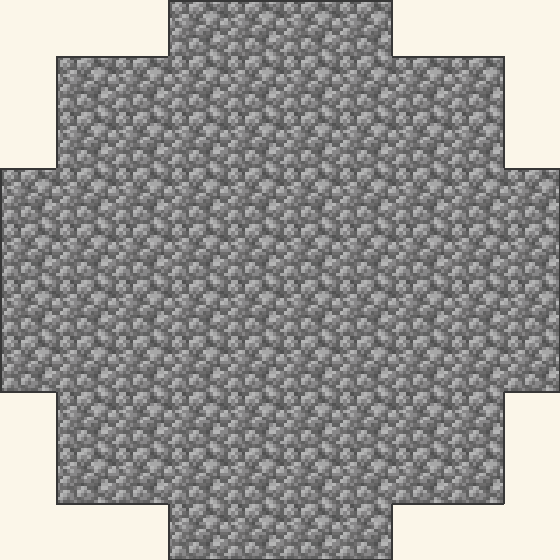
\includegraphics[width=\linewidth]{fig01_2d_d10_euclidean.png}
  \caption{\emph{Euclidiano}}
\end{subfigure}\hfill
\begin{subfigure}[t]{0.31\linewidth}\centering
  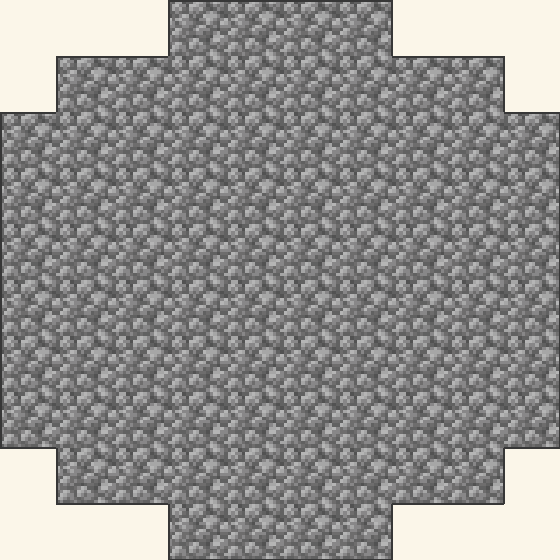
\includegraphics[width=\linewidth]{fig02_2d_d10_bresenham.png}
  \caption{\emph{Bresenham}}
\end{subfigure}\hfill
\begin{subfigure}[t]{0.31\linewidth}\centering
  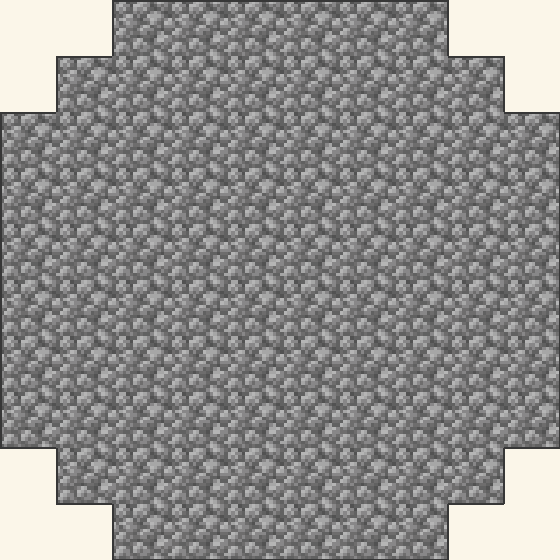
\includegraphics[width=\linewidth]{fig03_2d_d10_threshold.png}
  \caption{\emph{Limiar}}
\end{subfigure}
\caption{Mesma circunferencia de diametro 10 sob tres criterios de pertinencia, renderizada com a textura \emph{cobblestone} (pedregulho) do Minecraft. Observe como a celula de canto, a transicao entre linhas e os pontos cardeais variam de uma para outra --- sao tres respostas \emph{matematicamente corretas} sob criterios distintos, e tres planos de construcao diferentes em \emph{Minecraft}.}
\label{fig:comp-d10}
\end{figure}

\begin{nota}[Equidade e a realidade material da escola publica]
A escolha do Block Round responde, em parte, a um problema material concreto: a desigualdade de acesso a recursos digitais entre escolas publicas brasileiras. O Censo Escolar do INEP (2023) registra que somente 65\% das escolas publicas de Ensino Medio possuem laboratorio de informatica em funcionamento, com variacao regional acentuada. Por outro lado, o indice de posse de \emph{smartphones} pelos proprios estudantes e alto em todas as regioes (PNAD Continua TIC 2023 indica mais de 90\% entre jovens de 15--17 anos). O Block Round foi projetado para funcionar exatamente nesse cenario: \emph{smartphone} de baixo custo, sem internet permanente, sem cadastro --- e, quando necessario, o Apendice~\ref{ap:adapt-analog} oferece um itinerario \emph{totalmente analogico} para uso exclusivo de papel quadriculado. \emph{O proprio Minecraft, em sua versao Pocket Edition, roda em celulares de tres anos de uso}: o aluno pode comecar com Block Round na aula e continuar em casa no Minecraft.
\end{nota}

\begin{minec}[Pesquisa: Minecraft na educacao brasileira]
Pesquisas brasileiras recentes documentam o uso pedagogico de Minecraft em diversas redes: BITTENCOURT e GIRAFFA (\emph{Anais do Workshop sobre Jogos e Entretenimento Digital --- SBGames}, varios numeros) discutem o uso de Minecraft em ensino de algoritmica; FRANCISCO, REZENDE e colegas registram experiencias com Minecraft em aulas de matematica em escolas estaduais paulistas e mineiras; a \emph{Microsoft Educacao} mantem repositorio de planos de aula em portugues no portal \emph{Minecraft Education Edition} (\url{https://education.minecraft.net/pt-br}). Esta sequencia complementa essa tradicao: usa Block Round como \emph{ponte} para Minecraft, dispensando a instalacao do jogo (e a consequente exigencia de licenca, Java, ou conta Microsoft) no momento da aula.
\end{minec}

% =============================================================================
\section{Objetivos}\label{sec:objetivos}

\subsection{Objetivo geral}

Conduzir os estudantes a \acc{compreender, comparar, utilizar e traduzir-em-construcao} as definicoes formais da circunferencia, da elipse e do elipsoide como criterios de inclusao de celulas em uma malha discreta de voxels texturizados, mobilizando a equacao implicita dessas figuras para explicar, prever, modificar e \emph{construir no Minecraft} producoes visuais autorais, em dialogo com o patrimonio cultural visual brasileiro (modernismo, arte concreta, grafismo dos povos originarios) e com a tradicao matematica nacional. A consciencia dessa multiplicidade de respostas validas conecta-se a uma cultura matematica brasileira que, em 2014, viu \hyperref[sec:obmep]{Artur Avila} tornar-se o primeiro latino-americano a receber a Medalha Fields, e a uma cultura ludica em que comunidades brasileiras de \emph{Minecraft} ja constroem cidades inteiras articulando geometria espacial cotidianamente, sem necessariamente nomea-la.

\subsection{Objetivos especificos}

\textbf{Cognitivos (conceituais):}
\begin{itemize}[leftmargin=1.3em,itemsep=0.2em,topsep=0.3em]
  \item identificar a equacao implicita $\left(\dfrac{x}{r_x}\right)^{\!2} + \left(\dfrac{y}{r_y}\right)^{\!2} = 1$ como caso geral que contem a circunferencia $x^2 + y^2 = r^2$;
  \item reconhecer que tres criterios distintos de pertinencia (distancia no centro, ponto medio de Bresenham, cobertura de quina) produzem tres conjuntos diferentes de celulas --- como ja visto na Figura~\ref{fig:comp-d10};
  \item compreender a transicao da equacao 2D para a equacao 3D do elipsoide e relaciona-la com o calculo de volume $V = \tfrac{4}{3}\pi r_x r_y r_z$ (assunto recorrente no ENEM, eixo \emph{Geometria});
  \item interpretar o corte de um solido por um plano como uma \emph{desigualdade linear} aplicada as coordenadas dos voxels;
  \item compreender a \emph{aritmetica do inventario Minecraft} (stacks de 64, baus simples de 27 slots, baus duplos de 54 slots) como aplicacao concreta de \emph{divisao com teto} e \emph{representacao de quociente e resto};
  \item identificar as \emph{simetrias} (reflexao, rotacao) que permitem construir uma esfera completa a partir de um octante via \cmd{/clone}.
\end{itemize}

\textbf{Procedimentais:}
\begin{itemize}[leftmargin=1.3em,itemsep=0.2em,topsep=0.3em]
  \item operar a interface do Block Round em ambos os modos (2D e 3D) e exportar imagens em PNG e schematics em \texttt{.schem};
  \item desenhar manualmente, em papel quadriculado, a aproximacao discreta de uma circunferencia aplicando o criterio euclidiano e verifica-la no software;
  \item calcular a area/volume discreta de uma figura voxelizada contando celulas e comparar com a area/volume continua, expressando o resultado como erro relativo;
  \item compor uma figura autoral combinando circulos, elipses e elipsoides com justificativa matematica das escolhas, prevendo o numero de blocos por tipo e a quantidade de baus duplos necessaria;
  \item importar um schematic exportado pelo Block Round no Litematica ou Schematica (mods Minecraft) e executar a construcao no jogo;
  \item escrever uma sequencia de comandos \cmd{/clone} que reflita 1 octante em uma esfera completa.
\end{itemize}

\textbf{Atitudinais:}
\begin{itemize}[leftmargin=1.3em,itemsep=0.2em,topsep=0.3em]
  \item cooperar em duplas ou trios na producao das atividades praticas, simulando equipes de \emph{builders} de servidor Minecraft;
  \item argumentar matematicamente em defesa de uma escolha estetica --- competencia diretamente cobrada na redacao do ENEM e em discussoes orais de iniciacao cientifica;
  \item reconhecer que problemas reais (incluindo o problema de \enquote{construir uma cupula de Quartzo no servidor da turma}) admitem mais de uma resposta tecnicamente correta;
  \item identificar referencias matematicas no patrimonio cultural brasileiro, nos saberes ancestrais e na producao digital contemporanea (\emph{builders} de servidor, streamers, redes de Minecraft);
  \item desenvolver \emph{etica digital}: respeitar o trabalho dos colegas, citar a fonte de \emph{builds} reutilizadas, compreender o conceito de licenca.
\end{itemize}

% =============================================================================
\section{Competencias e habilidades da BNCC}\label{sec:bncc}

A sequencia mobiliza diretamente \acc{quatro habilidades} da area de Matematica e suas Tecnologias do Ensino Medio, alem de articular-se com o Tema Contemporaneo Transversal \emph{Cultura Digital} e com habilidades de Linguagens, Ciencias da Natureza e Ciencias Humanas.

\begin{habilidade}[EM13MAT307]
Empregar diferentes metodos para a obtencao da medida da area de uma superficie (reconfiguracoes, aproximacao por cortes etc.) e \acc{deduzir expressoes} de calculo para aplica-las em situacoes reais, \emph{com ou sem apoio de tecnologias digitais}.
\end{habilidade}

\begin{habilidade}[EM13MAT309]
Resolver e elaborar problemas que envolvem o \acc{calculo de areas totais e de volumes} de prismas, piramides e \emph{corpos redondos} em situacoes reais, \emph{com ou sem apoio de tecnologias digitais}.
\end{habilidade}

\begin{habilidade}[EM13MAT308]
Aplicar as relacoes metricas, incluindo as leis do seno e do cosseno ou as nocoes de congruencia e semelhanca, para resolver e elaborar problemas que envolvem triangulos em variados contextos.
\end{habilidade}

\begin{habilidade}[EM13MAT404]
Analisar funcoes definidas por uma ou mais sentencas, em suas representacoes algebrica e grafica, identificando dominios de validade, imagem, crescimento e decrescimento, \acc{convertendo essas representacoes de uma para outra}, com ou sem apoio de tecnologias digitais.
\end{habilidade}

\medskip
Mobilizam-se ainda as \emph{competencias especificas} de Matematica:

\begin{itemize}[leftmargin=1.3em,itemsep=0.15em,topsep=0.3em]
  \item \acc{Competencia 3} --- construir modelos para resolver problemas, analisando a plausibilidade dos resultados;
  \item \acc{Competencia 4} --- utilizar com flexibilidade diferentes registros de representacao matematicos (algebrico, geometrico, computacional, voxel);
  \item \acc{Competencia 5} --- investigar e estabelecer conjecturas empregando estrategias e tecnologias diversas.
\end{itemize}

\subsection{Articulacao com o ENEM}\label{sec:enem}

As habilidades acima conectam-se com os seguintes \emph{descritores} da Matriz de Referencia do ENEM:

\begin{itemize}[leftmargin=1.3em,itemsep=0.15em,topsep=0.3em]
  \item Competencia de Area 2 (\emph{Utilizar o conhecimento geometrico para realizar a leitura e a representacao da realidade}), com destaque para H7 (geometria plana), H8 (medidas) e H9 (volumes e areas);
  \item Competencia de Area 3 (\emph{Construir nocoes de variacao de grandezas para a compreensao da realidade e a solucao de problemas do cotidiano}), descritor H12;
  \item Competencia de Area 5 (\emph{Modelar e resolver problemas que envolvem variaveis socioeconomicas ou tecnico-cientificas, usando representacoes algebricas}), descritor H21.
\end{itemize}

A matriz oficial pode ser consultada no portal do \href{https://www.gov.br/inep/}{INEP}, na secao \emph{Avaliacao e Exames Educacionais} $\rightarrow$ \emph{ENEM}.

\subsection{Tema Contemporaneo Transversal}

O TCT \acc{Cultura Digital} atravessa toda a sequencia. Discutem-se questoes de \emph{etica digital} (licencas de software livre \emph{vs.} proprietario; a propria Mojang/Microsoft permite uso educacional gratuito do Minecraft via \emph{Education Edition}), \emph{protecao de dados pessoais} (\href{https://www.planalto.gov.br/ccivil_03/_ato2015-2018/2018/lei/l13709.htm}{LGPD, Lei 13.709/2018}), \emph{producao autoral} (direitos sobre as criacoes dos estudantes na Aula~\ref{aula5}) e \emph{cidadania digital} (comportamento responsavel em servidores Minecraft, prevencao de \emph{griefing} e bullying online).

% =============================================================================
\section{Conteudos}\label{sec:conteudos}

\subsection{Conceituais}
\begin{itemize}[leftmargin=1.3em,itemsep=0.15em,topsep=0.3em]
  \item Plano cartesiano e sistema de coordenadas em $\mathbb{R}^2$ e $\mathbb{R}^3$; centro de uma celula \emph{vs.} canto.
  \item Equacao reduzida da circunferencia: $x^2 + y^2 = r^2$.
  \item Equacao implicita geral da elipse: $\left(\dfrac{x}{r_x}\right)^{\!2} + \left(\dfrac{y}{r_y}\right)^{\!2} = 1$.
  \item Desigualdade da pertinencia: \emph{interior, exterior} e \emph{fronteira}.
  \item Equacao do elipsoide e da esfera em $\mathbb{R}^3$.
  \item Volume continuo do elipsoide: $V = \tfrac{4}{3}\pi r_x r_y r_z$.
  \item Planos no espaco como desigualdades lineares (operacao de corte).
  \item Vizinhanca de uma celula (4-conectada em 2D, 6-conectada em 3D).
  \item \acc{Aritmetica do inventario Minecraft}: stacks de 64; baus simples (27 slots) e duplos (54 slots); divisao com teto $N_{\mathrm{packs}} = \lceil N/64 \rceil$.
  \item \acc{Simetria octaedrica} e o grupo $\mathbb{Z}_2^3$ de reflexoes coordenadas (subgrupo de ordem 8 de $O_h$): aplicacao em construcao otimizada via \cmd{/clone}.
\end{itemize}

\subsection{Procedimentais}
\begin{itemize}[leftmargin=1.3em,itemsep=0.15em,topsep=0.3em]
  \item Tracado manual em papel quadriculado seguindo um criterio explicito.
  \item Operacao do Block Round (mudanca de modo, ajuste de \emph{sliders}, escolha de algoritmo, exportacao como PNG e \texttt{.schem}).
  \item Comparacao de areas/volumes discretos e continuos por contagem.
  \item Composicao de figuras combinadas (\emph{voxel art} autoral com fundamentacao geometrica).
  \item Importacao de \texttt{.schem} no Litematica/Schematica.
  \item Execucao de comandos vanilla \cmd{/fill}, \cmd{/clone}, \cmd{/setblock} e WorldEdit \cmd{//sphere}, \cmd{//hsphere}, \cmd{//ellipsoid}.
  \item Planejamento de coleta de recursos em modo survival.
\end{itemize}

\subsection{Atitudinais}
\begin{itemize}[leftmargin=1.3em,itemsep=0.15em,topsep=0.3em]
  \item Trabalho cooperativo em duplas ou trios.
  \item Argumentacao fundamentada (justificar escolhas com matematica).
  \item Etica digital: respeito a licenca do software, as producoes dos colegas e as regras do servidor Minecraft compartilhado.
  \item Valorizacao de referencias matematicas presentes em saberes brasileiros e na cultura \emph{gamer} contemporanea.
\end{itemize}

\subsection{Modos de renderizacao e variedade de algoritmos}

Alem de mudar o algoritmo, o Block Round oferece tres \emph{modos de renderizacao} (Preenchido, Fino, Grosso) que produzem visuais distintos para a mesma figura geometrica, como ilustra a Figura~\ref{fig:render-modes}. Em Minecraft, esses modos correspondem a tres tipos de construcao distintos: uma esfera \emph{Preenchida} usa todos os blocos do interior (uma cupula opaca de \emph{Stone}); \emph{Fina} mostra apenas a casca (uma cupula \emph{oca}, internamente vazia para uma sala ou museu); \emph{Grossa} fecha as fendas diagonais que o modo Fino deixa (\emph{essencial} para cupulas de \emph{Vidro} ou \emph{Gelo} subaquaticas que precisam ser estanques).

\begin{figure}[!htbp]
\centering
\begin{subfigure}[t]{0.31\linewidth}\centering
  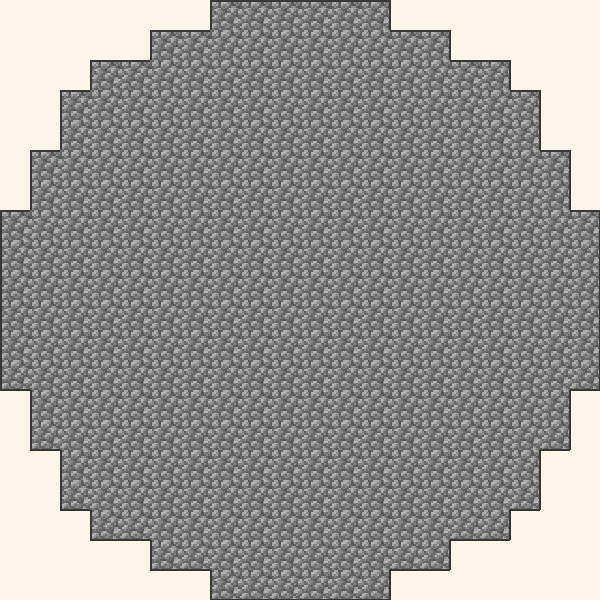
\includegraphics[width=\linewidth]{fig04_2d_d20_euclidean.png}
  \caption{\emph{Preenchido}}
\end{subfigure}\hfill
\begin{subfigure}[t]{0.31\linewidth}\centering
  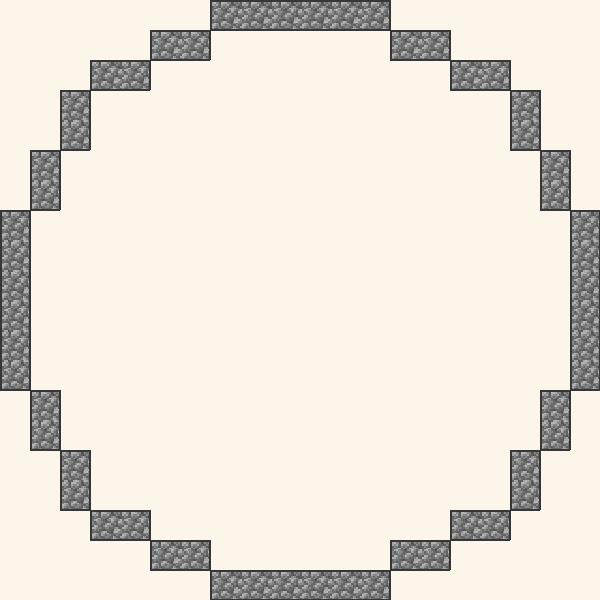
\includegraphics[width=\linewidth]{fig08_2d_d20_thin.png}
  \caption{\emph{Fino} (contorno de 1 bloco)}
\end{subfigure}\hfill
\begin{subfigure}[t]{0.31\linewidth}\centering
  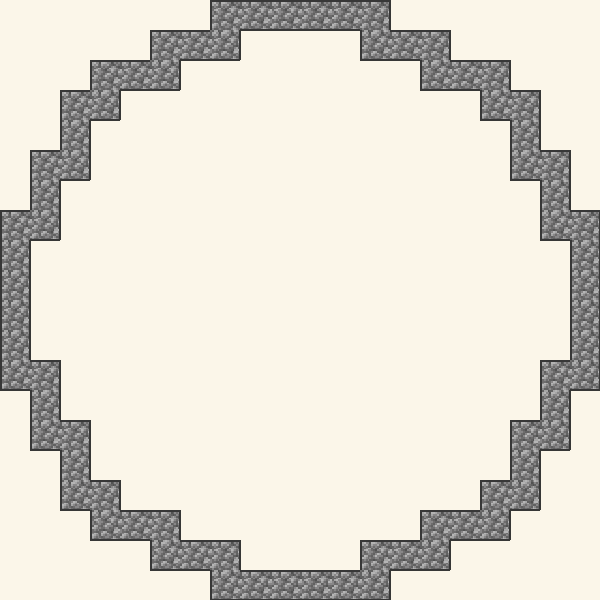
\includegraphics[width=\linewidth]{fig09_2d_d20_thick.png}
  \caption{\emph{Grosso} (contorno com pontes diagonais)}
\end{subfigure}
\caption{Os tres modos de renderizacao para a mesma circunferencia euclidiana de diametro 20. O modo \emph{Fino} corresponde ao bordo discreto topologico; o modo \emph{Grosso} adiciona blocos nas diagonais para evitar buracos a $45^\circ$ --- exatamente o problema que aparece em uma cupula de Vidro subaquatica do Minecraft, onde uma fenda diagonal deixa a agua entrar.}
\label{fig:render-modes}
\end{figure}

\subsection{Texturas de bloco: o diferencial Block Round}

Embora a matematica de \emph{quais voxels colocar} seja independente da textura, o Block Round renderiza cada voxel com sua textura canonica de seis faces do Minecraft. A mesma esfera de diametro 10 muda completamente de carater visual conforme o bloco escolhido (Figura~\ref{fig:textures}), \emph{sem nenhuma mudanca no algoritmo} subjacente. Esse e o ponto pedagogico central: a \emph{forma} e fruto da matematica, a \emph{aparencia} e uma decisao estetica posterior.

\begin{figure}[!htbp]
\centering
\begin{subfigure}[t]{0.31\linewidth}\centering
  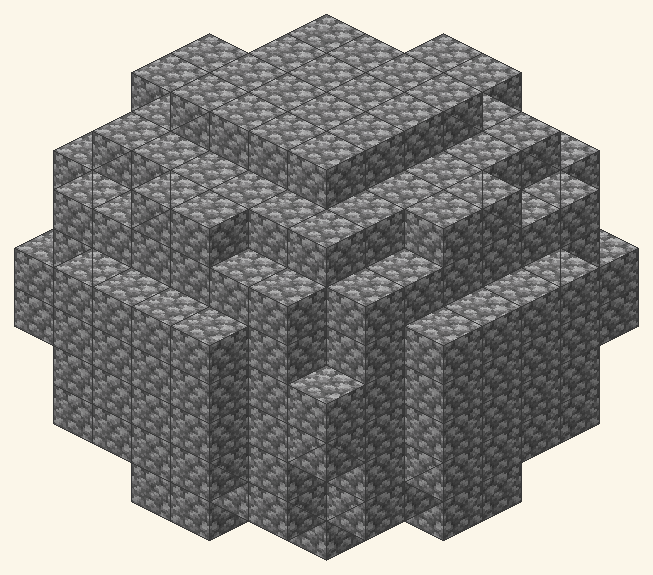
\includegraphics[width=\linewidth]{fig15_3d_sphere_cobblestone.png}
  \caption{\emph{Cobblestone}}
\end{subfigure}\hfill
\begin{subfigure}[t]{0.31\linewidth}\centering
  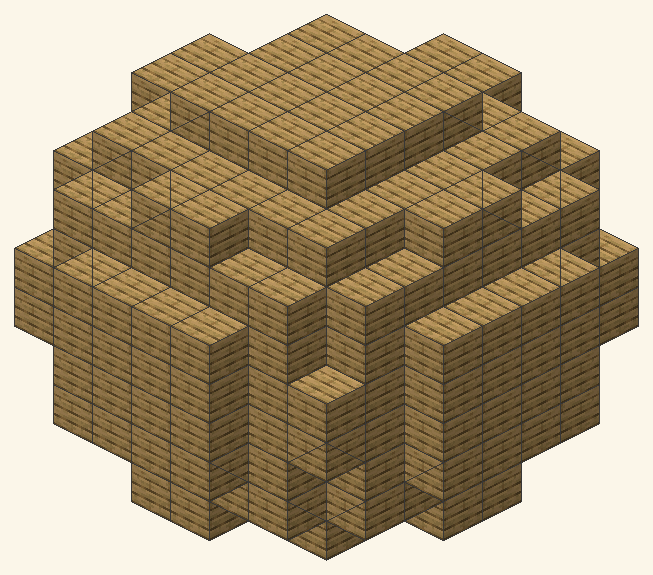
\includegraphics[width=\linewidth]{fig17_3d_sphere_oak.png}
  \caption{\emph{Oak Planks}}
\end{subfigure}\hfill
\begin{subfigure}[t]{0.31\linewidth}\centering
  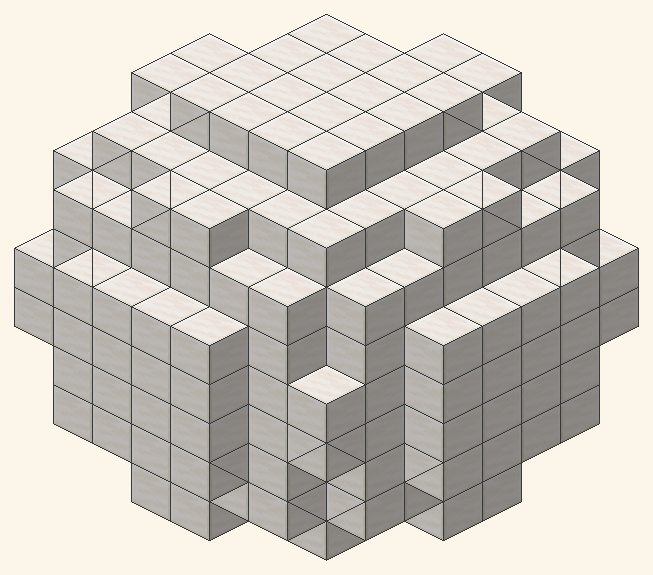
\includegraphics[width=\linewidth]{fig19_3d_sphere_quartz.png}
  \caption{\emph{Quartz Block}}
\end{subfigure}
\caption{Tres texturas Minecraft aplicadas a \emph{mesma} esfera de diametro 10. A silhueta voxelizada e identica nas tres versoes --- a matematica nao mudou. O que muda e o carater visual: \emph{Cobblestone} sugere muralha medieval, \emph{Oak Planks} sugere interior de cabana ou navio, \emph{Quartz Block} sugere templo moderno.}
\label{fig:textures}
\end{figure}

% =============================================================================
\section{Conhecimentos previos}\label{sec:prerrequisitos}

A sequencia pressupoe contato anterior com:

\begin{itemize}[leftmargin=1.3em,itemsep=0.15em,topsep=0.3em]
  \item Plano cartesiano: localizacao de pontos $(x, y)$ e $(x, y, z)$.
  \item Equacao reduzida da circunferencia (conteudo de 1.\textordmasculine\ ano EM).
  \item Areas de poligonos e do circulo; volumes de cubo, prisma e cilindro (conteudo de 2.\textordmasculine\ ano EM).
  \item Conceito de funcao: dominio, imagem, grafico.
  \item Nocao de proporcao e porcentagem.
  \item Divisao inteira com quociente e resto (Fundamental II).
\end{itemize}

\emph{Conhecimento previo opcional (nao requerido, mas util):} familiaridade com Minecraft. Esta sequencia foi propositalmente desenhada para que mesmo estudantes que \emph{nunca} jogaram Minecraft (situacao rara mas possivel, especialmente em escolas rurais com baixa conectividade) consigam acompanhar plenamente --- toda a operacao acontece no Block Round, que e \emph{auto-contido} no navegador.

Caso a turma demonstre defasagem em algum dos pontos obrigatorios acima --- realidade frequente no contexto pos-pandemia, conforme dados do \href{https://www.gov.br/inep/pt-br/areas-de-atuacao/avaliacao-e-exames-educacionais/saeb}{SAEB} 2023 que mostram queda nos indicadores de Matematica em diversas redes --- a \emph{Aula 1} dispoe de um momento de \emph{nivelamento diagnostico} (10 min) descrito em §\ref{aula1}.

% =============================================================================
\section{Recursos e materiais}\label{sec:recursos}

\subsection{Recursos digitais}
\begin{itemize}[leftmargin=1.3em,itemsep=0.15em,topsep=0.3em]
  \item Block Round (uma instancia por estudante \emph{ou} por dupla);
  \item Projetor multimidia, TV com entrada HDMI ou lousa digital interativa;
  \item Acesso a \emph{laboratorio de informatica} \emph{ou} uso de \emph{smartphones} pessoais (BYOD --- \emph{Bring Your Own Device}) \emph{ou} \emph{tablets} distribuidos por programas estaduais;
  \item (Opcional, Aula~\ref{aula5}) acesso a Minecraft Java Edition ou Minecraft Education Edition com mods \emph{Litematica} ou \emph{Schematica} instalados; alternativamente, uso vanilla com \cmd{/fill} e \cmd{/clone}.
\end{itemize}

\subsection{Recursos analogicos}
\begin{itemize}[leftmargin=1.3em,itemsep=0.15em,topsep=0.3em]
  \item Papel quadriculado (1\,cm), 2 folhas por estudante;
  \item Lapis preto, borracha, regua de 30\,cm;
  \item Lapis de cor ou canetinhas (preferencialmente verde-grama \texttt{\#5B8E3F} e marrom-terra \texttt{\#825432}, paleta Block Round);
  \item Folha de exercicios (Apendice~\ref{ap:exerc});
  \item Lousa convencional ou quadro branco.
\end{itemize}

\subsection{Livro didatico e PNLD}\label{sec:pnld}

O Block Round complementa --- nao substitui --- o livro didatico adotado pela escola via \href{https://www.gov.br/fnde/pt-br/acesso-a-informacao/acoes-e-programas/programas/programas-do-livro}{PNLD} (Programa Nacional do Livro e do Material Didatico). Colecoes recomendadas que cobrem os conteudos mobilizados:

\begin{itemize}[leftmargin=1.3em,itemsep=0.1em,topsep=0.2em,nosep]
  \item \emph{Matematica Contexto e Aplicacoes} (Luiz Roberto Dante), Atica;
  \item \emph{Matematica: Ciencia e Aplicacoes} (Iezzi, Dolce, Degenszajn, Perigo, Almeida), Saraiva;
  \item \emph{Matematica Paiva} (Manoel Paiva), Moderna;
  \item \emph{Conexoes com a Matematica} (Fabio Martins de Leonardo \emph{et al.}), Moderna.
\end{itemize}

Os capitulos sobre \emph{equacao da circunferencia}, \emph{conicas} e \emph{geometria espacial metrica} (volumes) dialogam diretamente com a sequencia. Em particular, problemas de \emph{ladrilhamento}, \emph{cobertura} e \emph{contagem em malhas} (comuns nos livros do PNLD) sao quase identicos ao problema central do Block Round, apenas com terminologia diferente.

\subsection{Acesso ao Block Round}

Em ordem de preferencia:

\begin{enumerate}[leftmargin=1.5em,itemsep=0.15em,topsep=0.3em]
  \item \textbf{Hospedado pelo professor} em \emph{GitHub Pages} ou no portal da escola (URL distribuida por QR Code projetado na lousa). Versao publica: \url{https://vinisouza128.github.io/block-round/}.
  \item \textbf{Copia local} dos arquivos do projeto em uma pasta do laboratorio, executada via \emph{file://}.
  \item \textbf{Offline em \emph{smartphone}} via PWA: basta abrir uma vez com internet para que o navegador instale o aplicativo.
\end{enumerate}

% =============================================================================
\section{Adaptacoes para a realidade plural brasileira}\label{sec:adapt}

A escola publica brasileira e heterogenea --- talvez a mais heterogenea do mundo entre redes nacionais. Esta sequencia foi desenhada para se adaptar a essa pluralidade, com variantes especificas para cada contexto.

\subsection{Escolas estaduais urbanas (capital ou regiao metropolitana)}
Cenario tipico de Sao Paulo, Belo Horizonte, Salvador, Fortaleza, Curitiba, Porto Alegre. Geralmente dispoe de laboratorio de informatica (uso compartilhado), lousa digital e Wi-Fi razoavel. Muitas redes ja licenciam \emph{Minecraft Education Edition} para alunos --- a Aula~\ref{aula5} pode ser feita integralmente nessa versao. \emph{Configuracao mais simples para implementar a sequencia integralmente em laboratorio.}

\subsection{Escolas estaduais urbanas (interior)}
Realidade da grande maioria dos municipios brasileiros. Laboratorio de informatica pode estar parcialmente operacional. Recomenda-se \emph{modelo BYOD} com \emph{smartphones} pessoais dos estudantes, organizados em duplas (um celular por dupla). O Block Round roda confortavelmente em \emph{Android} a partir de 2018. Se \emph{Minecraft} estiver indisponivel, a Aula~\ref{aula5} pode focar em comandos hipoteticos (papel + descricao do efeito) sem perder o conteudo conceitual. E a configuracao \acc{mais comum} no pais.

\subsection{Institutos Federais (IFs) e CEFETs}
Rede federal de excelencia tecnica. Geralmente bem equipada. A sequencia integra-se naturalmente aos cursos tecnicos integrados ao Ensino Medio (Informatica, Eletronica, Design Grafico, Multimidia, \emph{Mecatronica}). Recomenda-se aprofundar a Aula~\ref{aula2} (algoritmo de Bresenham) com implementacao em Python no laboratorio, e a Aula~\ref{aula5} com a instalacao real do servidor Minecraft Java no laboratorio para construcao colaborativa --- frequente em projetos de extensao dos IFs federais com escolas estaduais. Articula-se com o curso tecnico em \emph{Jogos Digitais} oferecido por varios IFs (IFRS Campus Porto Alegre, IFSC Campus Florianopolis, IFRN Campus Natal, IFMG Campus Bambui).

\subsection{Escolas do campo}
Cenario do PRONERA (Programa Nacional de Educacao na Reforma Agraria) e da Educacao do Campo. Tradicionalmente menos equipadas digitalmente, mas com \emph{forte conhecimento previo geometrico} dos estudantes (geometria aplicada a rocados, cercas, irrigacao por curvas de nivel, canteiros). Recomenda-se variante analogica (Apendice~\ref{ap:adapt-analog}) e dispositivo unico do professor para demonstracao. A Aula~\ref{aula3} pode aproveitar o conhecimento dos estudantes sobre construcao de currais circulares e silos de armazenamento para articular geometria vivida e geometria simbolica.

\subsection{Escolas indigenas e quilombolas}
A \href{https://www.planalto.gov.br/ccivil_03/_ato2007-2010/2008/lei/l11645.htm}{Lei 11.645/2008} estabelece a obrigatoriedade do ensino de historia e cultura afro-brasileira e indigena. Esta sequencia pode ser \emph{enriquecida com saberes proprios da comunidade}: a oca tradicional Tupi-Guarani (cobertura semi-elipsoidal de palha), a maloca Yanomami circular, o kijemy Yawalapiti (casa cerimonial de planta circular), o kilombo de Palmares (organizacao espacial circular concentrica). \emph{O professor de Arte e os ancioes da comunidade sao parceiros essenciais nessa adaptacao} (ver Aula~\ref{aula3}, Atividade~\ref{at:34}). Em servidor Minecraft, ja existem comunidades brasileiras que reconstroem aldeias indigenas tradicionais bloco a bloco --- referenciar pode ser util.

\subsection{Educacao de Jovens e Adultos (EJA)}
Tipicamente turmas noturnas, com estudantes adultos que retornam a escola. O Block Round funciona bem aqui porque a interface e amigavel e o tema (Minecraft / videogames) e tambem familiar a essa faixa etaria (varios adultos joveis cresceram com Minecraft a partir de 2011; outros aprenderam pelos filhos). Sugere-se reduzir o tempo de cada atividade em 20\% (em virtude do turno mais curto da EJA) e priorizar discussoes orais em vez de producao escrita longa. A Aula~\ref{aula5} pode ser tornada \emph{opcional} para EJA, focando-se nas Aulas 1--4.

\subsection{Variante para 2 aulas geminadas (100 min cada)}
Para escolas com horario em \emph{modulo duplo} (frequente em IFs e em projetos de tempo integral): Aulas 1+2 num modulo, 3+4 no outro, Aula 5 sozinha (ou em modulo simples de 50 min, ou em modulo duplo se houver tempo para construcao real). Total: 3 modulos de 100 min + 1 modulo de 50 min, ou 2 modulos de 100 min + 1 modulo duplo (200 min) para a parte pratica final em Minecraft.

\subsection{Crosswalk com Curriculos Referenciais Estaduais}

Cada secretaria estadual de educacao detalhou a BNCC em seu proprio curriculo referencial. As principais redes:

\begin{center}
\small
\begin{tabularx}{\textwidth}{@{}p{0.18\textwidth}p{0.25\textwidth}X@{}}
\toprule
\textbf{Rede} & \textbf{Curriculo de referencia} & \textbf{Habilidades equivalentes a EM13MAT307/309} \\
\midrule
SEDUC-SP & Curriculo Paulista (2020) & Bimestre de Geometria, 3.\textordmasculine\ EM, eixo \emph{Geometria e Medidas}. \\
\addlinespace[3pt]
SEEDUC-RJ & Curriculo Minimo Estadual & Unidade tematica \emph{Geometria espacial metrica}. \\
\addlinespace[3pt]
SEE-MG & Curriculo Referencia de MG & Eixo \emph{Geometria}, 3.\textordmasculine\ EM. \\
\addlinespace[3pt]
SEDUC-CE & DCRC (Documento Curricular Referencial do Ceara) & Geometria espacial metrica e analitica. \\
\addlinespace[3pt]
SEDUC-AM & Curriculo Referencia do Amazonas & Geometria com itinerario integrado a \emph{Aprofundamento em STEM}. \\
\addlinespace[3pt]
SEED-PR & Curriculo da Rede Estadual Paranaense & Geometria espacial; \emph{Pensamento Computacional} no Itinerario Formativo. \\
\bottomrule
\end{tabularx}
\end{center}

\subsection{Ensino hibrido ou remoto}
A natureza \emph{web} do Block Round o torna trivialmente compativel com aulas remotas (\emph{Google Meet}, \emph{Zoom}, plataformas estaduais como \emph{CMSP} de Sao Paulo ou \emph{Sala de Aula Digital} de outras redes). O professor compartilha sua tela; estudantes acompanham na propria maquina. As atividades em papel quadriculado podem ser fotografadas e enviadas como tarefa assincrona via WhatsApp do grupo da turma, Google Classroom ou plataforma da rede. A Aula~\ref{aula5} pode ser feita em servidor Minecraft compartilhado --- \emph{Realms} ou servidor proprio --- com a turma encontrando-se no mundo virtual e construindo colaborativamente.

% =============================================================================
\section{Sequencia didatica}\label{sec:sequencia}

A sequencia segue a estrutura \acc{mobilizacao --- problematizacao --- sistematizacao --- sintese}, inspirada nos \emph{tres momentos pedagogicos} de Delizoicov \& Angotti (1990) e na tradicao freireana de partir do conhecimento previo do estudante. Cada aula de 50 minutos respeita o ritmo cognitivo do adolescente, alternando momentos expositivos breves ($\leq 15$\,min) com atividades praticas.

% =============================================================================
\subsection{Aula 1 --- \enquote{Como o jogo desenha uma esfera com cubos?}}\label{aula1}

\subsubsection*{Objetivo da aula}
Estabelecer o \emph{problema central} da rasterizacao discreta como um problema matematico genuino, mobilizar a equacao da circunferencia e apresentar o Block Round. Reconhecer que o problema central da aula --- \emph{como decidir quais blocos pintar?} --- e exatamente o problema que cada jogador de Minecraft enfrenta ao construir uma esfera no jogo.

\begin{atividade}[1.1 --- Mobilizacao \quad\tempo{10 min}]
\textbf{Estrategia:} \emph{think--pair--share} (pensar individualmente, conversar em dupla, compartilhar com a turma). \\[0.4em]
\textbf{Passo a passo:}
\begin{enumerate}[leftmargin=1.5em,itemsep=0.2em,topsep=0.3em,nosep]
  \item Projetar (ou desenhar) tres construcoes classicas do Minecraft: uma cupula de Vidro sobre uma base de Stone (qualquer tutorial brasileiro no YouTube); a \emph{Esfera Gigante} construida coletivamente em um servidor brasileiro popular (\emph{Mineplex BR}, \emph{Hypixel}, ou um servidor caseiro de turma); o Pixel Art de um personagem brasileiro feito em Minecraft (Mascote da Copa, personagem de \emph{Turma da Monica}, \emph{Saci-Pere}, jogador de futebol).
  \item Perguntar a turma: \emph{\enquote{Olhem com atencao. Como o jogo decide quais cubos colocar para fazer uma esfera? O Minecraft tem um \enquote{compasso magico} embutido?}}
  \item Cada estudante anota individualmente sua resposta (1\,min) e em seguida discute com o colega ao lado (2\,min).
  \item Recolha coletiva: anotar respostas-chave no canto da lousa. Conduzir para a observacao fundamental: \emph{\enquote{O jogo so consegue colocar cubos inteiros --- como ele decide quais?}}
\end{enumerate}
\end{atividade}

\begin{atividade}[1.2 --- Problematizacao \quad\tempo{15 min}]
\textbf{Estrategia:} desenho manual confrontado com a definicao formal. \\[0.4em]
\textbf{Material:} papel quadriculado, lapis. \\[0.4em]
\textbf{Passo a passo:}
\begin{enumerate}[leftmargin=1.5em,itemsep=0.2em,topsep=0.3em,nosep]
  \item Cada estudante recebe meia folha de papel quadriculado e marca o ponto central de uma regiao $11 \times 11$ celulas.
  \item Comando: \emph{\enquote{Pintem o melhor circulo que voces conseguirem com diametro 10 (raio 5). \emph{Imaginem que cada quadradinho e um bloco de cobblestone do Minecraft.} Voces tem 4 minutos.}}
  \item Apos o tempo, tres ou quatro estudantes vao a lousa reproduzir seu desenho em uma malha desenhada com giz/marcador.
  \item Observacao dirigida pelo professor: \emph{\enquote{Olhem. Voces fizeram a mesma figura? Por que nao? Quem esta certo? Se cada um de voces estivesse construindo essa esfera num servidor Minecraft compartilhado, que problema isso geraria?}}
  \item Sistematizar: nao ha \emph{uma unica} resposta (a Figura~\ref{fig:comp-d10} apresentada na §\ref{sec:justificativa} corrobora). Cada estudante adotou implicitamente um \acc{criterio} diferente para decidir se uma celula entra ou nao.
\end{enumerate}

\textbf{Nota etnomatematica:} aproveitar o momento para mencionar que \emph{essa diversidade de respostas e exatamente o objeto da Etnomatematica} (Ubiratan D'Ambrosio), campo brasileiro reconhecido internacionalmente que estuda como diferentes culturas e grupos resolvem problemas matematicos de maneiras distintas e igualmente validas. \emph{A propria comunidade brasileira de Minecraft constitui um grupo cultural com \enquote{etnomatematica} propria}, transmitida por tutoriais em portugues no YouTube, por mods feitos por brasileiros, e por servidores nacionais como o \emph{Beasty Craft} e o \emph{LBoladao}.
\end{atividade}

\begin{atividade}[1.3 --- Sistematizacao \quad\tempo{15 min}]
\textbf{Estrategia:} exposicao dialogada com apoio do quadro. \\[0.4em]
\textbf{Conteudo:}

A equacao implicita da circunferencia centrada na origem de raio $r$ e

\begin{formula}
\centering
$\displaystyle x^2 + y^2 \;=\; r^2$
\end{formula}

Pontos \emph{dentro} satisfazem $x^2 + y^2 < r^2$; pontos \emph{fora}, $x^2 + y^2 > r^2$. A equacao se generaliza para a elipse de semi-eixos $r_x, r_y$:

\begin{formula}
\centering
$\displaystyle \left(\dfrac{x}{r_x}\right)^{\!2} + \left(\dfrac{y}{r_y}\right)^{\!2} \;=\; 1$
\end{formula}

Em uma malha de blocos (voxels), o desafio e decidir quais \acc{celulas} pertencem ao interior. Decisoes diferentes geram desenhos diferentes. O Block Round implementa \emph{tres} criterios:

\begin{itemize}[leftmargin=1.3em,itemsep=0.15em,topsep=0.3em]
  \item \acc{Euclidiano}: o centro $(i + \tfrac{1}{2},\, j + \tfrac{1}{2})$ da celula esta dentro?
  \item \acc{Bresenham}: algoritmo historico de 1965, opera apenas com inteiros.
  \item \acc{Limiar}: alguma \emph{quina} da celula esta dentro?
\end{itemize}

\textbf{Demonstracao:} o professor abre o Block Round, ajusta o diametro para 10, alterna entre os tres algoritmos com a turma observando as diferencas. Sublinhar: as tres figuras sao \emph{matematicamente corretas} sob criterios distintos. Mostrar que o app permite trocar a textura do bloco --- a esfera passa a ser de cobblestone, oak\_planks, diamond, glowstone, e a forma \emph{nao muda}. \emph{Esse e o ponto central de Block Round: a forma e matematica, a textura e escolha estetica.}
\end{atividade}

\begin{atividade}[1.4 --- Sintese \quad\tempo{10 min}]
\textbf{Estrategia:} aplicacao imediata individual. \\[0.4em]
\textbf{Comando:} \emph{\enquote{Voltem ao papel. Refacam o circulo de diametro 10 aplicando \acc{rigorosamente} o criterio euclidiano: pintar a celula se, e somente se, o ponto central dela $(i + 0{,}5,\, j + 0{,}5)$ estiver a uma distancia menor ou igual a 5 do centro.}}

Ao final, comparar o desenho do papel com o que o Block Round produz no algoritmo Euclidiano com diametro 10 --- a referencia visual e a Figura~\ref{fig:comp-d10}~(a). \emph{Devem coincidir.}
\end{atividade}

\begin{minec}[Conexao com o jogo]
Em \emph{Minecraft Java Edition} com o mod WorldEdit instalado, o comando \cmd{//sphere stone 5} desenha exatamente a mesma figura que o Block Round produz no algoritmo \emph{Bresenham} com diametro 10. Estudantes que joguem em servidores podem confirmar isso em casa --- as construcoes sao identicas. \emph{Ou seja: o que estamos estudando na aula nao e uma simulacao didatica do Minecraft; e a mesma matematica que o jogo usa.}
\end{minec}

\subsubsection*{Tarefa de casa (opcional)}
Repetir o exercicio 1.4 com diametros 8 e 14. Trazer os tres desenhos na aula seguinte. Para quem joga Minecraft em casa: tentar reproduzir o desenho diretamente no jogo (com \cmd{/setblock} bloco a bloco, ou com \cmd{//sphere} se tiver WorldEdit) e fotografar a construcao.

% =============================================================================
\subsection{Aula 2 --- \enquote{Tres algoritmos, tres desenhos, tres planos de construcao}}\label{aula2}

\subsubsection*{Objetivo da aula}
Aprofundar a compreensao dos tres algoritmos como definicoes matematicas distintas e comparar quantitativamente os resultados, incluindo o impacto pratico em termos de \emph{numero de blocos a coletar} para um construtor de survival.

\begin{atividade}[2.1 --- Retomada \quad\tempo{5 min}]
Recolher rapidamente os desenhos da tarefa de casa, observar variacoes na turma, anunciar o objetivo da aula: \emph{\enquote{Hoje vamos olhar para cada um dos tres algoritmos com lupa, e descobrir por que Bresenham e considerado uma joia da Computacao --- e por que a comunidade Minecraft brasileira, sem nunca ter ouvido falar dele, ja o usa todo dia.}}
\end{atividade}

\begin{atividade}[2.2 --- Algoritmo Euclidiano \quad\tempo{10 min}]
Formalizacao. Para uma celula $(i, j)$, calcular as coordenadas normalizadas

\begin{formula}
\centering
$\displaystyle d_x = \dfrac{i + \tfrac{1}{2} - c_x}{r_x},\qquad d_y = \dfrac{j + \tfrac{1}{2} - c_y}{r_y}$
\end{formula}

A celula e pintada se, e somente se, $d_x^{\,2} + d_y^{\,2} \leq 1$.

\textbf{No quadro:} resolver explicitamente o caso $c_x = c_y = 5$, $r_x = r_y = 5$, celula $(2, 1)$. Tem-se $d_x = (2{,}5 - 5)/5 = -0{,}5$ e $d_y = (1{,}5 - 5)/5 = -0{,}7$, portanto $d_x^2 + d_y^2 = 0{,}25 + 0{,}49 = 0{,}74 \leq 1$. Celula \emph{dentro}. \\

Pedir aos estudantes que testem a celula $(0, 0)$ (qual o resultado?). Discutir.
\end{atividade}

\begin{atividade}[2.3 --- Algoritmo de Bresenham \quad\tempo{15 min}]\label{at:23}
\textbf{Contexto historico:} Jack Bresenham publicou o algoritmo em 1965 quando trabalhava na IBM. Antes dele, tracar uma reta exigia operacoes em ponto flutuante --- caras nos computadores da epoca. Bresenham mostrou que era possivel desenhar usando \emph{apenas inteiros}: somas e comparacoes.

A versao para circunferencia usa um \emph{parametro de decisao} $d$. Comeca-se em $(x{=}0,\, y{=}R)$ com $d_0 = 1 - R$. A cada passo no octante $0$--$45^\circ$:

\begin{formula}
\centering
$\begin{cases}
\text{se } d < 0: & \text{proximo: } (x{+}1,\, y),\; d \mathrel{+}= 2x+3 \\
\text{se } d \geq 0: & \text{proximo: } (x{+}1,\, y{-}1),\; d \mathrel{+}= 2(x-y)+5
\end{cases}$
\end{formula}

\textbf{Demonstracao no quadro:} tracar passo a passo o algoritmo para $R = 5$, anotando $x, y, d$ a cada iteracao. Os oito octantes sao obtidos por simetria. \\

\textbf{Conexao com Minecraft:} o algoritmo \cmd{//sphere} do mod \emph{WorldEdit} (Sponge, Bukkit, Paper, Fabric) implementa uma variante de Bresenham 3D --- a mesma matematica de 1965, agora rodando em milhoes de servidores Minecraft pelo mundo. \emph{O que voce esta aprendendo agora e o que o jogo usa por baixo dos panos toda vez que alguem digita \texttt{//sphere stone 8}.}

\textbf{Conexao com a OBI:} o algoritmo de Bresenham e tema classico em provas da \href{https://olimpiada.ic.unicamp.br/}{Olimpiada Brasileira de Informatica (OBI)}, organizada pela SBC (Sociedade Brasileira de Computacao) na Unicamp. Estudantes interessados podem aprofundar via o material gratuito disponivel no portal da OBI.

\textbf{Observacao metodologica:} se a turma demonstrar dificuldade com a algebra do parametro $d$, basta apresentar o algoritmo como uma \emph{regra} (sem demonstrar a funcao de decisao). A justificacao completa esta no documento tecnico \texttt{Block\_Round\_Math\_pt-BR.pdf}, §5.
\end{atividade}

\begin{atividade}[2.4 --- Algoritmo de Limiar \quad\tempo{10 min}]
Para cada celula $(i, j)$, identificar a \emph{quina mais proxima} do centro da forma:

\begin{formula}
\centering
$\displaystyle n_x = \mathrm{clamp}(c_x,\, i,\, i{+}1),\qquad n_y = \mathrm{clamp}(c_y,\, j,\, j{+}1)$
\end{formula}

A celula e incluida se $\left(\dfrac{n_x - c_x}{r_x}\right)^{\!2} + \left(\dfrac{n_y - c_y}{r_y}\right)^{\!2} \leq 0{,}94$.

\textbf{Por que $0{,}94$ e nao $1$?} Empiricamente, com $1$ aparecem \enquote{espinhos} de 1 bloco nos pontos cardeais. O limiar levemente menor elimina o artefato. \emph{Esta e uma decisao de engenharia tomada por inspecao visual} --- um exemplo importante de como a matematica teorica nem sempre basta sozinha. Em termos freireanos: a \enquote{palavra final} nao e da formula, mas do dialogo entre teoria e pratica.

\textbf{Quando usar Limiar em Minecraft:} para cupulas e domos vistos \emph{de longe} (templo no topo de uma montanha, mausoleu em ilha), o algoritmo Limiar produz uma silhueta levemente mais \enquote{cheia} que le melhor atraves de neblina e oclusao ambiente. Custo: $\sim$\,5--10\% mais blocos por casca. Recomendado para projetos onde a estetica vista de longe importa mais do que economia de material.
\end{atividade}

\begin{atividade}[2.5 --- Comparacao quantitativa \quad\tempo{10 min}]\label{at:25}
\textbf{Atividade pratica em duplas.} No Block Round (ou no projetor centralizado):
\begin{enumerate}[leftmargin=1.5em,itemsep=0.15em,topsep=0.3em,nosep]
  \item Definir diametro 20 e modo \emph{Preenchido} (a Figura~\ref{fig:comp-d20} mostra o resultado esperado para cada algoritmo).
  \item Acionar o \emph{Info chip} no canto do canvas. Anotar a area de cada um dos tres algoritmos.
  \item Calcular a area continua: $\pi r^2 = \pi \cdot 10^2 \approx 314{,}16$.
  \item Para cada algoritmo, calcular o erro relativo: $\dfrac{|\text{area discreta} - \text{area continua}|}{\text{area continua}} \times 100\%$.
  \item Ordenar os tres algoritmos do mais proximo ao mais distante do valor continuo.
  \item \emph{Conexao com Minecraft:} \enquote{\emph{Se voces fossem construir essas tres esferas em survival, qual exigiria menos viagens ao deposito de cobblestone? Qual exigiria mais?}} A diferenca em pacotes (\emph{stacks}) de 64 blocos pode chegar a 1 pacote inteiro entre o algoritmo de menor area (Euclidiano) e o de maior area (Limiar).
\end{enumerate}

\textbf{Resultado esperado:} Euclidiano costuma ficar muito proximo (erro abaixo de $2\%$); Limiar sobreestima em poucos por cento; Bresenham fica no meio. Confirmar coletivamente.
\end{atividade}

\begin{figure}[!htbp]
\centering
\begin{subfigure}[t]{0.31\linewidth}\centering
  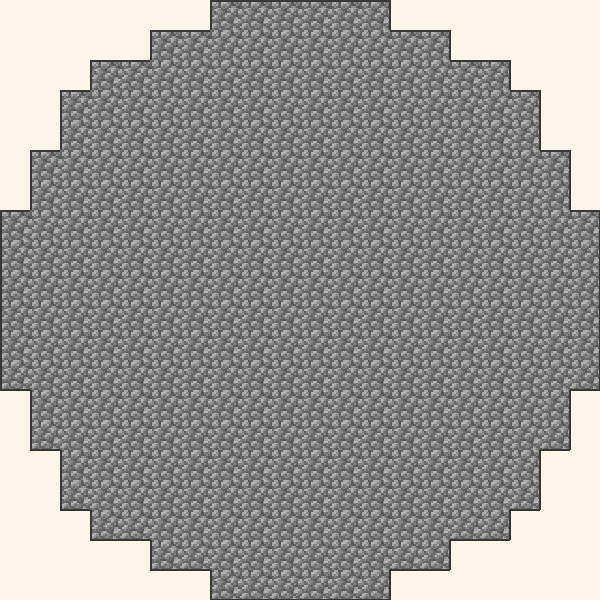
\includegraphics[width=\linewidth]{fig04_2d_d20_euclidean.png}
  \caption{\emph{Euclidiano}}
\end{subfigure}\hfill
\begin{subfigure}[t]{0.31\linewidth}\centering
  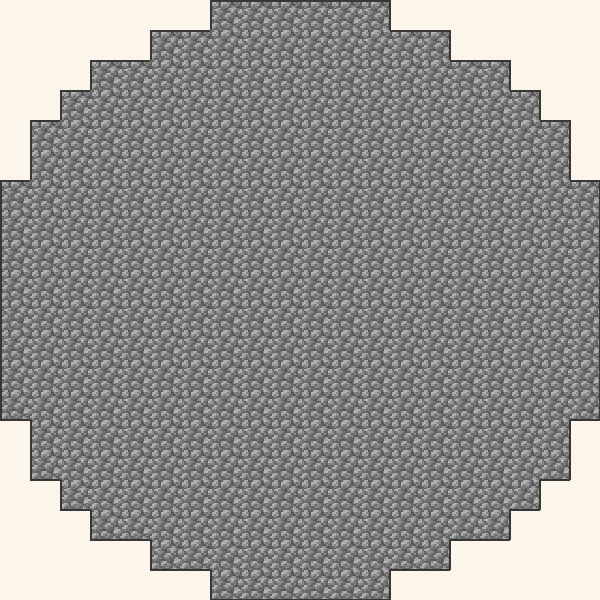
\includegraphics[width=\linewidth]{fig05_2d_d20_bresenham.png}
  \caption{\emph{Bresenham}}
\end{subfigure}\hfill
\begin{subfigure}[t]{0.31\linewidth}\centering
  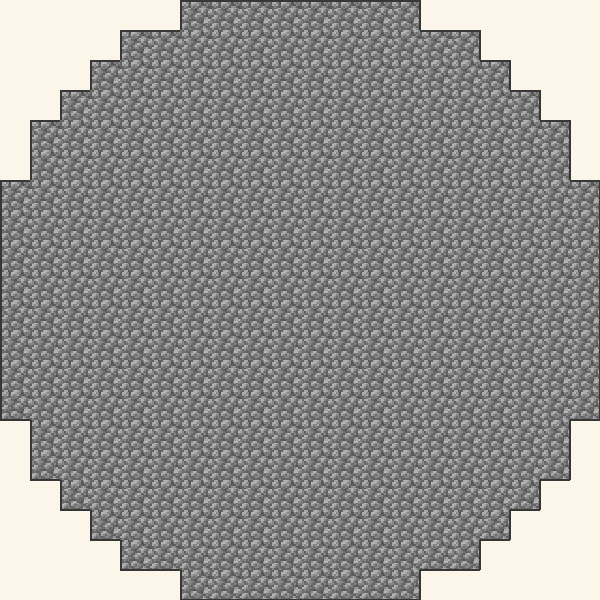
\includegraphics[width=\linewidth]{fig06_2d_d20_threshold.png}
  \caption{\emph{Limiar}}
\end{subfigure}
\caption{Mesma circunferencia de diametro 20 nos tres algoritmos, renderizada com a textura cobblestone. O aumento de diametro torna as diferencas mais sutis --- as tres versoes parecem semelhantes a olho nu. E um bom momento para comentar que para diametros pequenos (Figura~\ref{fig:comp-d10}) as diferencas sao muito mais evidentes.}
\label{fig:comp-d20}
\end{figure}

\begin{minec}[Comparacao de blocos: Block Round \emph{vs.} WorldEdit]
Tente em casa (se tiver Minecraft + WorldEdit): execute \cmd{//sphere stone 10} num servidor e conte os blocos. Compare com o que o Block Round informa no \emph{Info chip} para algoritmo Bresenham, $D = 20$. As duas contagens devem coincidir (\emph{ou} diferir por 0--4 blocos por causa de pequenas diferencas de implementacao). Se voce achar uma diferenca consistente, voce descobriu uma curiosidade matematica genuina.
\end{minec}

% =============================================================================
\subsection{Aula 3 --- \enquote{Da elipse ao elipsoide: a terceira dimensao}}\label{aula3}

\subsubsection*{Objetivo da aula}
Generalizar a equacao da elipse para o elipsoide, introduzir voxels, calculo de volume discreto e cortes planares. Estabelecer pontes com a tradicao visual brasileira e com construcoes famosas da comunidade Minecraft brasileira.

\begin{atividade}[3.1 --- Da equacao 2D para 3D \quad\tempo{15 min}]\label{at:31}
Acrescentar uma terceira coordenada $z$ ao plano cartesiano. A equacao implicita da elipse generaliza-se naturalmente:

\begin{formula}
\centering
$\displaystyle \left(\dfrac{x}{r_x}\right)^{\!2} + \left(\dfrac{y}{r_y}\right)^{\!2} + \left(\dfrac{z}{r_z}\right)^{\!2} \;=\; 1$
\end{formula}

Quando $r_x = r_y = r_z = r$, recupera-se a \acc{esfera} $x^2 + y^2 + z^2 = r^2$, como ilustrado na Figura~\ref{fig:3d-shapes}.

\textbf{Voxels:} a celula de uma malha 3D chama-se \emph{voxel} (\emph{volume element}). Em Minecraft, cada voxel corresponde a um \emph{bloco} de $1\times1\times1$. O criterio de pertinencia e exatamente o mesmo do caso 2D, acrescido da coordenada $z$:

\begin{formula}
\centering
$\displaystyle a_x^2 + a_y^2 + a_z^2 \leq 1,\quad \text{com } a_\xi = \dfrac{\xi + \tfrac{1}{2} - c_\xi}{r_\xi}$
\end{formula}

\textbf{Demonstracao:} abrir o Block Round no modo 3D, alternar entre Esfera e Elipsoide, rotacionar com o \emph{mouse}, observar a estrutura de voxels.
\end{atividade}

\begin{figure}[!htbp]
\centering
\begin{subfigure}[t]{0.45\linewidth}\centering
  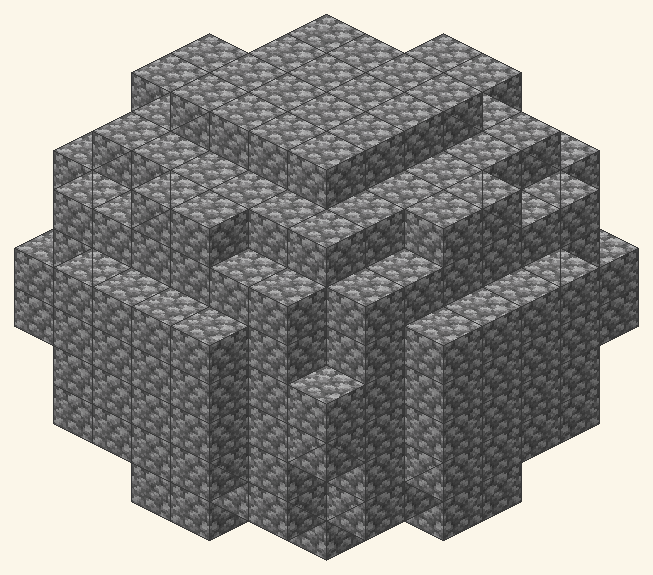
\includegraphics[width=\linewidth]{fig10_3d_sphere_d12.png}
  \caption{Esfera de diametro 10 ($r_x = r_y = r_z = 5$).}
\end{subfigure}\hfill
\begin{subfigure}[t]{0.45\linewidth}\centering
  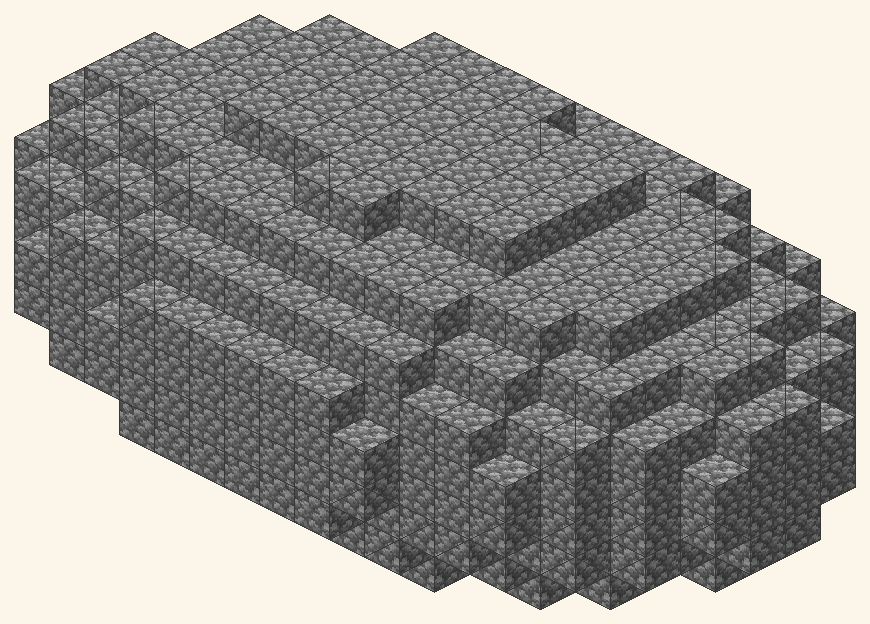
\includegraphics[width=\linewidth]{fig11_3d_ellipsoid.png}
  \caption{Elipsoide com $W = 20, H = 10, D = 12$.}
\end{subfigure}
\caption{Voxelizacao em 3D. Cada cubo e um voxel (= bloco de Minecraft); sua coordenada $(i, j, k)$ no centro e testada na equacao implicita. As escadarias visiveis na superficie sao caracteristicas da voxelizacao --- exatamente o aspecto que da ao Minecraft sua identidade visual.}
\label{fig:3d-shapes}
\end{figure}

\begin{atividade}[3.2 --- Volume continuo \emph{vs.} discreto \quad\tempo{15 min}]\label{at:32}
O volume continuo do elipsoide e um resultado classico:

\begin{formula}
\centering
$\displaystyle V \;=\; \dfrac{4}{3}\,\pi\, r_x\, r_y\, r_z$
\end{formula}

Quando $r_x = r_y = r_z = r$, $V = \tfrac{4}{3}\pi r^3$. Este e um conteudo \acc{recorrente no ENEM} (questoes de Geometria Espacial cobradas em praticamente todas as edicoes) e tambem na fase 2 da \hyperref[sec:obmep]{OBMEP}, especialmente em problemas que envolvem aproximacao numerica.

\textbf{Atividade em dupla:}
\begin{enumerate}[leftmargin=1.5em,itemsep=0.15em,topsep=0.3em,nosep]
  \item Calcular o volume continuo de uma esfera de diametro 12 ($r = 6$): $V = \tfrac{4}{3}\pi \cdot 216 \approx 904{,}78$.
  \item No Block Round, gerar a esfera $D = 12$, modo \emph{Preenchido}, acionar \emph{Info chip}, anotar o volume discreto (numero de blocos): aproximadamente $V_{\mathrm{disc}} \approx 904$ blocos. \emph{Erro relativo $\approx 0{,}1\%$ --- impressionante.}
  \item No mesmo chip, observar a notacao \emph{$904 = 14 \times 64 + 8$}: o jogo dira ao construtor de survival \enquote{voce precisa de \emph{14 stacks completos} de cobblestone + uma stack parcial com \emph{8 blocos}}.
  \item Repetir para $D = 16$ ($V_{\mathrm{cont}} \approx 2\,144$; $V_{\mathrm{disc}} \approx 2\,145$). Notar que para $D$ par o erro pode ate ser \emph{positivo} (sobreestimacao por causa do centro entre celulas).
\end{enumerate}

\textbf{Observacao:} a relacao $\text{volume discreto}/\text{volume continuo} \to 1$ quando $D \to \infty$. Para $D$ pequeno, ha divergencia sensivel --- e isso e matematicamente correto: a discretizacao \emph{de fato} altera a contagem.
\end{atividade}

\begin{atividade}[3.3 --- Cortes planares \quad\tempo{10 min}]\label{at:33}
O Block Round permite cortar o elipsoide por tres planos diferentes. Cada corte e uma \acc{desigualdade linear} aplicada ao centro do voxel:

\begin{formula}
\centering
$\begin{array}{lcl}
\text{Eixo X:} & x \geq \mathit{cut} & \Rightarrow \text{voxel descartado} \\
\text{Eixo Y:} & y \geq \mathit{cut} & \Rightarrow \text{voxel descartado} \\
\text{Diagonal:} & x + y \geq \mathit{cut} & \Rightarrow \text{voxel descartado}
\end{array}$
\end{formula}

A Figura~\ref{fig:cortes} ilustra os tres cortes a $50\%$.

\textbf{Discussao dirigida:} \emph{\enquote{Por que um corte diagonal tem amplitude $D_x + D_y$ e nao $D_x$? Onde esta a hipotenusa?}} Conduzir para o reconhecimento de que $x + y$ assume valores entre $0$ e $D_x + D_y$ na caixa retangular. \emph{No Minecraft, um corte Y 50\% em uma esfera produz uma \enquote{cupula} classica --- a metade superior da esfera, que e exatamente a construcao que cobre templos, observatorios e arenas em milhares de servidores.}
\end{atividade}

\begin{figure}[!htbp]
\centering
\begin{subfigure}[t]{0.31\linewidth}\centering
  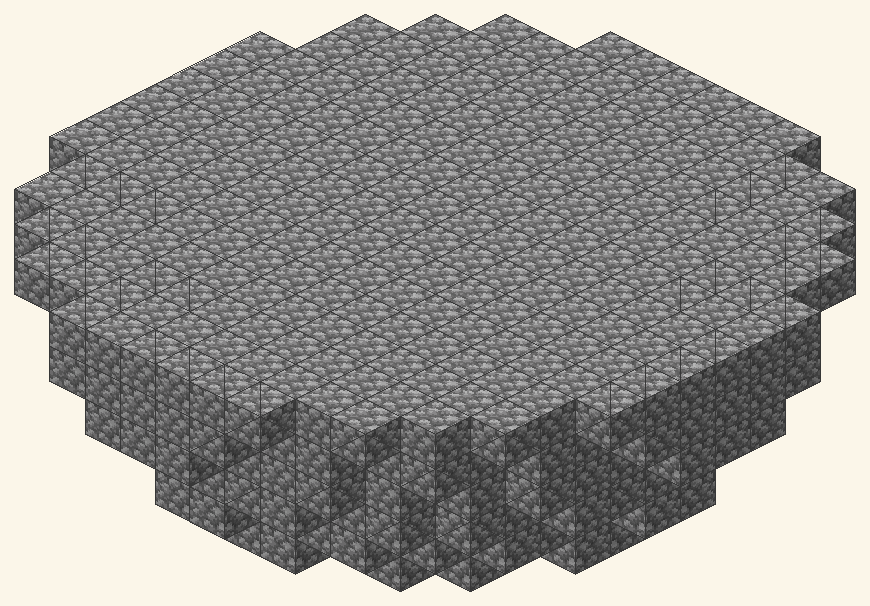
\includegraphics[width=\linewidth]{fig12_3d_cut_y50.png}
  \caption{Corte Y a 50\% --- a \emph{cupula} classica.}
\end{subfigure}\hfill
\begin{subfigure}[t]{0.31\linewidth}\centering
  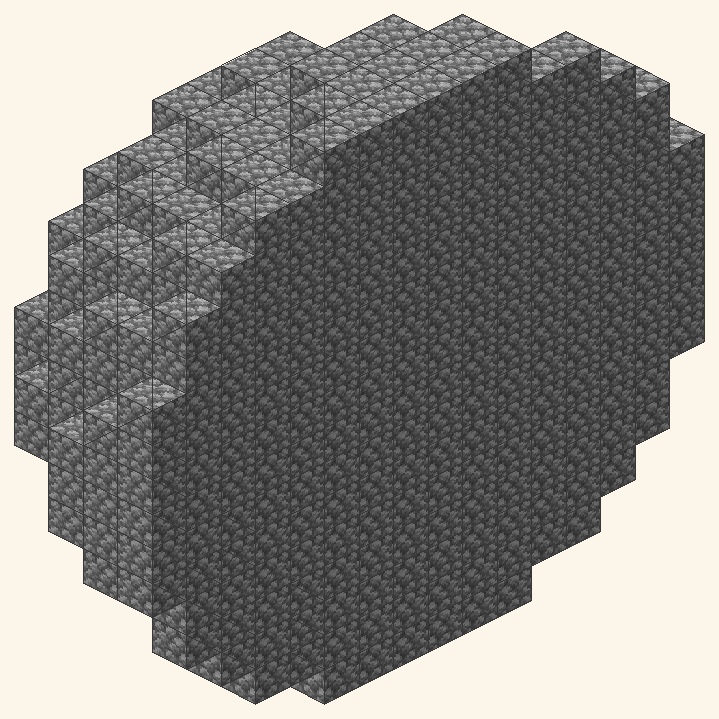
\includegraphics[width=\linewidth]{fig13_3d_cut_x50.png}
  \caption{Corte X a 50\% --- uma \emph{meia-esfera lateral}.}
\end{subfigure}\hfill
\begin{subfigure}[t]{0.31\linewidth}\centering
  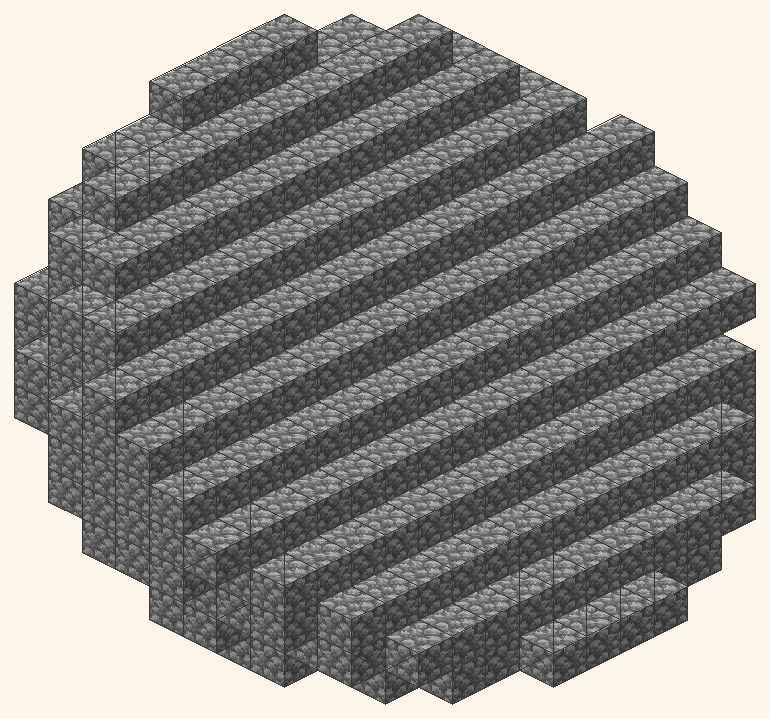
\includegraphics[width=\linewidth]{fig14_3d_cut_diag50.png}
  \caption{Corte diagonal a 50\% --- uma \emph{meia-bacia} oblqua.}
\end{subfigure}
\caption{Tres cortes planares no mesmo elipsoide de diametro 16, todos preservando $50\%$ do volume. Observe o padrao escalonado caracteristico do corte diagonal: ele expoe a hipotenusa que conecta os dois eixos. Cada corte e um plano de construcao Minecraft diferente: cupula de templo, meia-arena lateral, anfiteatro de fonte.}
\label{fig:cortes}
\end{figure}

\begin{atividade}[3.4 --- Dialogo com o patrimonio visual brasileiro \quad\tempo{10 min}]\label{at:34}
\emph{Conexao com Linguagens, Arte e Historia. Esta atividade cumpre as competencias da BNCC sobre identidade cultural e patrimonio.}

Projetar (ou distribuir impressas) cinco imagens:

\begin{itemize}[leftmargin=1.3em,itemsep=0.2em,topsep=0.3em,nosep]
  \item \acc{Catedral Metropolitana de Brasilia} (Oscar Niemeyer, 1970): suas 16 colunas curvas constituem um \emph{hiperboloide de revolucao} construido com concreto armado. Junto com o Palacio do Itamaraty, o Memorial JK e o MAC Niteroi (este ultimo abertamente elipsoidal, ver Figura~\ref{fig:3d-shapes}(b)), Niemeyer realizou em escala arquitetonica exatamente as quadricas que estamos estudando.

  \item \acc{Oca Tupi-Guarani / Maloca Yanomami / Kijemy Yawalapiti}: as casas tradicionais dos povos originarios brasileiros frequentemente tem planta circular ou semi-elipsoidal. Saberes arquitetonicos transmitidos oralmente ao longo de seculos contem geometria sofisticada --- \emph{voxelizacao}, ainda que sem o nome.

  \item \acc{Grafismo Kadiweu} (MS): os desenhos corporais e em ceramica do povo Kadiweu, descritos por Claude Levi-Strauss em \emph{Tristes Tropicos} (1955), sao reconhecidos por sua sofisticacao geometrica: \emph{simetrias dobradas}, particao do espaco em zonas circulares e quadrangulares justapostas. Tradicao matematica viva, anterior a colonizacao.

  \item \acc{Ceramica marajoara} (PA, seculos V--XIV): vasos e estatuetas com motivos circulares concentricos, espirais e divisoes geometricas. Patrimonio arqueologico brasileiro reconhecido pelo IPHAN.

  \item \acc{Builds da comunidade brasileira de Minecraft}: cidades construidas em servidores como \emph{LBoladao}, \emph{Beasty Craft}, \emph{Cubocraft}, ou nos servidores escolares. Pode-se mostrar timelapses de constructions de cupulas, esferas e arcos publicados no YouTube brasileiro. \emph{Esta e a etnomatematica de Minecraft brasileira em acao}, contemporanea, viva, em portugues.
\end{itemize}

\textbf{Discussao dirigida:} \emph{\enquote{Niemeyer projetou em concreto as mesmas curvas que voces desenharam em blocos. Os povos Kadiweu e marajoaras representaram circulos e simetrias usando barro, tinta corporal e tecido --- seculos antes dos computadores existirem. A comunidade Minecraft brasileira faz isso ao vivo, todos os dias, em servidores compartilhados. O problema da rasterizacao que estudamos nao e uma invencao da era digital: e uma constante da historia humana. Cada cultura encontrou seu modo de \emph{rasterizar}.}}

\textbf{Articulacao interdisciplinar:} parceria sugerida com o(a) professor(a) de Arte, de Historia e/ou de Geografia para aprofundamento. A Aula~\ref{aula4} e a Aula~\ref{aula5} podem pedir que os grupos \emph{escolham} qual tradicao visual brasileira inspirara seu trabalho.
\end{atividade}

% =============================================================================
\subsection{Aula 4 --- \enquote{Aritmetica do inventario: stacks, baus, comandos}}\label{aula4}

\subsubsection*{Objetivo da aula}
Introduzir a \emph{aritmetica de inventario} de Minecraft como aplicacao concreta de divisao com teto e representacao de quociente e resto. Apresentar os comandos centrais (\cmd{/fill}, \cmd{/clone}, \cmd{//sphere}, \cmd{//hsphere}) e a otimizacao por simetria octaedrica.

\begin{atividade}[4.1 --- Aritmetica de stacks \quad\tempo{15 min}]\label{at:41}
Em Minecraft, cada slot do inventario carrega no maximo \acc{64 blocos identicos}. Esse limite e o que da significado pratico ao calculo de volume: $V = 904$ blocos para uma esfera $D=12$ \emph{nao} significa \enquote{$904$ na maleta} --- significa \enquote{$\lceil 904/64 \rceil = 15$ \emph{stacks} (slots cheios)} de cobblestone.

\textbf{Formulas chaves:}

\begin{formula}
\centering
$\displaystyle N_{\mathrm{stacks}} = \left\lceil \dfrac{V}{64} \right\rceil
\qquad\qquad
N_{\mathrm{baus\,duplos}} = \left\lceil \dfrac{V}{3\,456} \right\rceil$
\end{formula}

(Um bau simples tem 27 slots; um bau duplo, 54 slots; $54 \times 64 = 3\,456$ itens por bau duplo.)

\textbf{Atividade em dupla:}
\begin{enumerate}[leftmargin=1.5em,itemsep=0.15em,topsep=0.3em,nosep]
  \item Para uma esfera $D = 8$ (volume $\approx 268$ blocos): quantos stacks? Quantos baus simples? Resposta: 5 stacks; 1 bau simples (com 17 slots livres).
  \item Para uma esfera $D = 16$ (volume $\approx 2\,145$ blocos): quantos stacks? Quantos baus duplos? Resposta: 34 stacks; 1 bau duplo (faltam 20 stacks para encher --- ou seja, sobra para mais um cilindro pequeno).
  \item Para uma esfera $D = 32$ (volume $\approx 17\,156$ blocos): quantos stacks? Quantos baus duplos? Resposta: 269 stacks (que e $\approx 5$ baus duplos $+$ 1 stack), $\lceil 17\,156/3\,456 \rceil = 5$ baus duplos.
  \item \emph{No Minecraft, em modo survival, mineradores brasileiros tipicamente extraem 1 stack de cobblestone a cada 4--6 minutos (depende da pickaxe). Calcular o tempo total estimado de coleta para a esfera $D = 16$: $34 \times 5 = 170$ minutos $\approx 2{,}8$ horas.}
\end{enumerate}
\end{atividade}

\begin{atividade}[4.2 --- Comandos Minecraft \quad\tempo{15 min}]\label{at:42}
Apresentar os comandos centrais:

\begin{itemize}[leftmargin=1.4em,itemsep=0.25em,topsep=0.3em]
  \item \cmd{/setblock x y z minecraft:stone} --- coloca um bloco em uma posicao especifica.
  \item \cmd{/fill x1 y1 z1 x2 y2 z2 minecraft:stone} --- preenche uma caixa retangular com um bloco. Limite vanilla: $32\,768$ blocos por comando.
  \item \cmd{/clone x1 y1 z1 x2 y2 z2 x3 y3 z3} --- copia uma regiao para outra posicao (poder fundamental para construcao por simetria).
  \item \cmd{//sphere stone 8} (WorldEdit) --- desenha uma esfera de raio 8 centrada no jogador, usando algoritmo Bresenham 3D.
  \item \cmd{//hsphere stone 8} (WorldEdit) --- desenha uma esfera \emph{oca} (apenas casca). Util para cupulas vazias por dentro.
  \item \cmd{//ellipsoid stone 10 5 10} (WorldEdit) --- elipsoide $W = 20, H = 10, D = 20$ com semi-eixos especificados.
\end{itemize}

\textbf{Demonstracao (se houver Minecraft disponivel):} executar \cmd{//sphere stone 8} num mundo de testes e cronometrar. Comparar com o que o Block Round mostra para diametro 16, algoritmo Bresenham. Confirmar a identidade matematica das duas saidas.

\textbf{Se nao houver Minecraft:} executar mentalmente. Anotar em papel quadriculado: \enquote{Estou no chao (y=64). Quero uma esfera de raio 8 a partir de y=72 (8 blocos acima do chao). Qual comando?} Resposta: \cmd{//sphere stone 8} estando em $(0, 72, 0)$.
\end{atividade}

\begin{atividade}[4.3 --- Otimizacao por simetria octaedrica \quad\tempo{15 min}]\label{at:43}
\textbf{Ideia central:} uma esfera centrada na origem e invariante por reflexoes nos tres planos coordenados. O grupo $\mathbb{Z}_2^3$ tem ordem 8: a partir de um \emph{octante} (regiao $+x, +y, +z$), as outras sete regioes sao obtidas por reflexao.

\textbf{Implicacao pratica:} em vez de colocar $V$ blocos um a um, construir $V/8$ blocos no octante positivo e refletir 7 vezes com \cmd{/clone}.

\begin{formula}
\centering
$\displaystyle \mathrm{custo}_\mathrm{simetria} = N_\mathrm{octante} + 7\, T_\mathrm{clone}
\;\ll\; \mathrm{custo}_\mathrm{forca\,bruta} = N\, T_\mathrm{bloco}$
\end{formula}

\textbf{Exemplo concreto, esfera $D = 24$ centrada em $(0, 72, 0)$:}
\begin{enumerate}[leftmargin=1.5em,itemsep=0.15em,topsep=0.3em,nosep]
  \item Construir manualmente o octante positivo ($\approx 905$ blocos, $\approx 15$ minutos em survival ou $\approx 45$ segundos em creative com brush).
  \item Refletir em $-x$: \cmd{/clone 0 72 0 12 84 12 -12 72 0 mode:masked}
  \item Refletir em $-y$: \cmd{/clone 0 72 0 12 84 12 0 60 0 mode:masked}
  \item Refletir em $-z$: \cmd{/clone 0 72 0 12 84 12 0 72 -12 mode:masked}
  \item Octantes $(-x, -y)$, $(-y, -z)$, $(-x, -z)$, $(-x, -y, -z)$: comandos analogos.
\end{enumerate}

\textbf{Comparacao de tempo:}
\begin{itemize}[leftmargin=1.3em,itemsep=0.1em,topsep=0.2em,nosep]
  \item Sem simetria, em survival: $7\,238$ blocos $\times$ 2s/bloco $\approx$ 4 horas.
  \item Com simetria: 15 min (octante) + 0,5s (7 clones) $\approx$ 15 min.
  \item Aceleracao: \emph{fator 16}.
\end{itemize}
\end{atividade}

\begin{atividade}[4.4 --- Aplicacao: planejamento de uma cupula real \quad\tempo{5 min}]
Em duplas, planejar (\emph{no papel ou no Block Round}) a construcao de uma cupula de Quartz $D=20$ em cima de um templo Maya/marajoara/Niemeyer estilizado. Anotar:
\begin{itemize}[leftmargin=1.3em,itemsep=0.1em,topsep=0.2em,nosep]
  \item Volume da cupula (metade da esfera $D=20$): $\approx 2\,094$ blocos.
  \item Stacks necessarias: 33 stacks.
  \item Numero de Quartz blocks (cada um exige 4 Nether Quartz, mineraveis no Nether): $\sim 2\,094 \times 4 = 8\,376$ Nether Quartz.
  \item Sequencia de comandos otimizada usando simetria.
\end{itemize}

Esta atividade prepara o terreno para a Aula 5 (construcao real).
\end{atividade}

% =============================================================================
\subsection{Aula 5 --- \enquote{Construcao real: do Block Round ao Minecraft}}\label{aula5}

\subsubsection*{Objetivo da aula}
Mobilizar todo o conteudo desenvolvido em um \emph{produto autoral construido}: exportar do Block Round, importar no Minecraft (via Litematica ou Schematica), executar a construcao em creative ou survival. Avaliar aprendizagem por meio da defesa argumentativa das escolhas matematicas e da entrega do produto final.

\begin{atividade}[5.1 --- Apresentacao do desafio \quad\tempo{5 min}]\label{at:51}
\textbf{Comando:} \emph{\enquote{Em duplas ou trios, voces vao produzir uma construcao em Minecraft (ou em Block Round, se nao houver Minecraft disponivel) que combine, no minimo, tres figuras geradas pelo Block Round (circulos, elipses, esferas ou elipsoides). Pode ser uma cidade no servidor da turma, um templo, uma fazenda redonda, um observatorio --- escolham voces. Ao final, cada grupo apresentara a obra explicando \acc{matematicamente} as escolhas: por que esse algoritmo? por que essa proporcao? por que esse corte? por que esses blocos?}}
\end{atividade}

\begin{atividade}[5.2 --- Exportacao e importacao \quad\tempo{15 min}]\label{at:52}
Demonstrar o fluxo Block Round $\rightarrow$ Minecraft:

\begin{enumerate}[leftmargin=1.5em,itemsep=0.2em,topsep=0.3em]
  \item No Block Round, configurar a figura desejada (p.ex.\ esfera $D = 12$ de Quartz com cut Y 50\%).
  \item Clicar no botao \emph{Exportar Schematic} no canto do canvas. O arquivo \texttt{.schem} (Sponge Schematic v2) e baixado.
  \item No Minecraft Java Edition com mod \emph{Litematica} instalado (gratuito): abrir o mod, \emph{Load Schematic}, selecionar o arquivo baixado.
  \item O Litematica mostra um \enquote{fantasma} translucido da construcao na posicao que o jogador escolher.
  \item O jogador coloca cada bloco \emph{seguindo o fantasma}. Litematica destaca em vermelho qualquer bloco fora do lugar.
  \item \emph{Alternativa via \cmd{//schem load}:} em servidor com WorldEdit, \cmd{//schem load nome\_arquivo} importa o schematic, e \cmd{//paste -a} cola na posicao atual --- construcao instantanea.
\end{enumerate}

\textbf{Se nao houver Minecraft disponivel:} demonstrar a exportacao do \texttt{.schem} e exibir o arquivo binario com um editor hexadecimal --- discussao sobre formato Sponge v2, gzip, NBT. Itinerario formativo de Computacao.
\end{atividade}

\begin{atividade}[5.3 --- Producao \quad\tempo{20 min}]\label{at:53}
\textbf{Material por grupo:}
\begin{itemize}[leftmargin=1.3em,itemsep=0.15em,topsep=0.3em,nosep]
  \item Acesso ao Block Round (computador ou \emph{smartphone});
  \item (Opcional) Acesso ao Minecraft com Litematica ou Schematica;
  \item Papel quadriculado, lapis e canetinhas para esbocos e roteiro;
  \item Folha-roteiro com tres questoes obrigatorias (Apendice~\ref{ap:exerc}, exercicio 8).
\end{itemize}

\textbf{Etapas internas do trabalho de grupo:}
\begin{enumerate}[leftmargin=1.5em,itemsep=0.15em,topsep=0.3em,nosep]
  \item \tempo{5 min} Brainstorm e esboco em papel.
  \item \tempo{8 min} Producao no Block Round e exportacao do \texttt{.schem}.
  \item \tempo{5 min} Importacao no Minecraft e teste rapido (se disponivel).
  \item \tempo{2 min} Redacao da justificativa matematica no roteiro.
\end{enumerate}

\textbf{Acompanhamento docente:} circular entre os grupos, fazendo perguntas mediadoras --- \emph{\enquote{Por que voces escolheram esse algoritmo? Como esse corte poderia ser descrito por uma desigualdade? Quantos baus duplos de Quartz voces vao precisar?}}
\end{atividade}

\begin{atividade}[5.4 --- Apresentacao e sintese coletiva \quad\tempo{10 min}]\label{at:54}
Cada grupo dispoe de 2 minutos para apresentar a obra a turma, mostrando-a no projetor (ou no Minecraft, ou fisicamente em papel) e respondendo \emph{ao menos a uma} das tres questoes matematicas exigidas.

\textbf{Criterios minimos da apresentacao:}
\begin{itemize}[leftmargin=1.3em,itemsep=0.1em,topsep=0.2em,nosep]
  \item identificar pelo menos uma figura matematica presente;
  \item nomear o algoritmo escolhido e justificar (mesmo \emph{a posteriori}) por que ele se adequa ao efeito visual pretendido;
  \item se houver corte 3D, descreve-lo como desigualdade;
  \item estimar (mesmo grosseiramente) o numero de stacks/baus necessarios.
\end{itemize}

\textbf{Sintese final pelo professor (3 min):} retomar a ideia central da sequencia --- \emph{\enquote{em uma malha discreta de voxels, a mesma curva continua admite multiplas representacoes; escolher uma e tomar uma decisao matematica; construir aquilo em Minecraft e tomar uma decisao de cidadania, gestao de recursos e estetica}} --- e situa-la no horizonte da matematica brasileira contemporanea: convidar a turma a explorar a \hyperref[sec:obmep]{OBMEP}, a saber mais sobre Artur Avila, e a participar de servidores Minecraft brasileiros que promovam construcoes colaborativas.
\end{atividade}

\begin{minec}[Possibilidades de extensao]
Esta Aula 5 abre varias possibilidades de extensao em projetos extra-classe:
\begin{itemize}[leftmargin=1.3em,itemsep=0.15em,topsep=0.3em,nosep]
  \item \textbf{Projeto Cidade Matematica:} a turma constroi uma cidade no servidor escolar, onde cada predio implementa uma figura geometrica (cilindro, esfera, elipsoide, conjunto de conicas).
  \item \textbf{Recriacao do patrimonio brasileiro:} reconstrucao em Minecraft da Catedral de Brasilia, do MAC Niteroi, do Pao de Acucar, do Cristo Redentor (com elipsoides!), ou de uma oca Tupi-Guarani.
  \item \textbf{Olimpiada Block Round:} competicao interna --- quem constroi a esfera mais proxima do volume continuo? quem otimiza melhor o tempo via simetria?
  \item \textbf{Articulacao com Engenharia (IFs/CEFETs):} usar o Block Round como sandbox de pre-engenharia: cupulas geodesicas, treliças voxelizadas, structures que aproximam superficies suaves.
  \item \textbf{Articulacao com Programacao (OBI):} reimplementar os tres algoritmos em Python ou Scratch, comparar saidas com Block Round, submeter analise como projeto de iniciacao cientifica.
\end{itemize}
\end{minec}

% =============================================================================
\section{Avaliacao}\label{sec:avaliacao}

A avaliacao adota o modelo \acc{formativo}, \acc{processual} e \acc{somativo}, articulando quatro dimensoes (mais uma dimensao especifica para a aplicacao em Minecraft) e dialogando com a tradicao brasileira da avaliacao por habilidades (Sanmarti, 2007; Luckesi, 1990).

\subsection{Avaliacao diagnostica}
Realizada na Aula~\ref{aula1}, no momento da Atividade~1.2 (desenho manual do circulo). Permite ao professor identificar dificuldades com plano cartesiano, equacao da circunferencia e contagem --- e contornar lacunas pos-pandemicas evidenciadas pelo SAEB 2023.

\subsection{Avaliacao formativa}
Distribuida pelas cinco aulas: observacao direta da participacao, qualidade das respostas no \emph{think--pair--share}, correcao \emph{imediata} dos calculos das Atividades~\ref{at:25}, \ref{at:32} e~\ref{at:41}.

\subsection{Avaliacao somativa}
Composta por duas entregas:

\begin{enumerate}[leftmargin=1.5em,itemsep=0.2em,topsep=0.3em,nosep]
  \item \textbf{Lista de exercicios} (Apendice~\ref{ap:exerc}), 8 questoes, entregue ao final da Aula~\ref{aula5} ou em data combinada.
  \item \textbf{Projeto final} (Atividade~\ref{at:53}), com roteiro respondido na defesa (Atividade~\ref{at:54}).
\end{enumerate}

\subsection{Rubrica de avaliacao}

\begin{center}
\small
\begin{tabularx}{\textwidth}{@{}p{0.21\textwidth}XX@{}}
\toprule
\textbf{Dimensao} & \textbf{Plenamente satisfatorio (8--10)} & \textbf{Parcialmente satisfatorio (5--7) / Insuficiente (0--4)} \\
\midrule
\textbf{Conceitos matematicos} & Aplica corretamente a equacao implicita da elipse/elipsoide; reconhece os tres criterios algoritmicos e suas diferencas. & Aplica equacao basica da circunferencia mas confunde-se com a generalizacao para elipse / nao reconhece as diferencas algoritmicas. \\
\addlinespace[3pt]
\textbf{Uso do software (Block Round)} & Opera o Block Round com autonomia em 2D e 3D; exporta imagens e \texttt{.schem}; alterna algoritmos e estilos. & Necessita de auxilio frequente; opera apenas 2D. \\
\addlinespace[3pt]
\textbf{Argumentacao} & Justifica matematicamente as escolhas no projeto final; usa vocabulario tecnico apropriado (\emph{algoritmo}, \emph{voxel}, \emph{corte}, \emph{desigualdade}, \emph{stack}, \emph{bau duplo}). & Justifica esteticamente, sem mobilizar a matematica; vocabulario ausente. \\
\addlinespace[3pt]
\textbf{Aplicacao pratica Minecraft} & Calcula corretamente stacks e baus para o projeto; descreve sequencia de comandos \cmd{/fill} ou \cmd{//sphere}; usa simetria octaedrica. & Confunde quociente e resto; trata blocos como unidades soltas; nao usa simetria. \\
\addlinespace[3pt]
\textbf{Cooperacao} & Trabalha produtivamente em dupla/trio; contribui com a discussao coletiva. & Trabalha isoladamente; pouca contribuicao. \\
\bottomrule
\end{tabularx}
\end{center}

\subsection{Conversao para notas}
\begin{itemize}[leftmargin=1.3em,itemsep=0.1em,topsep=0.2em,nosep]
  \item Lista de exercicios: 40\% da nota.
  \item Projeto final + apresentacao: 50\% da nota.
  \item Observacao processual (participacao): 10\% da nota.
\end{itemize}

% =============================================================================
\section{Articulacoes com o ecossistema matematico brasileiro}\label{sec:obmep}

A sequencia se insere em um \emph{ecossistema rico} de iniciativas brasileiras de educacao e pesquisa em matematica e tecnologia, que o professor pode mobilizar como ampliacao ou aprofundamento.

\subsection{OBMEP --- Olimpiada Brasileira de Matematica das Escolas Publicas}

Fundada em 2005 e organizada pelo \acc{IMPA} (Instituto de Matematica Pura e Aplicada) em parceria com a SBM (Sociedade Brasileira de Matematica), a \href{https://www.obmep.org.br/}{OBMEP} e a maior olimpiada de matematica do mundo: mais de 18 milhoes de estudantes inscritos a cada edicao, exclusivamente da rede publica.

\emph{O conteudo desta sequencia (geometria analitica do circulo e do elipsoide, raciocinio algoritmico, aproximacoes numericas) e diretamente preparatorio para questoes da Fase 2 da OBMEP do nivel 3 (Ensino Medio).}

\subsection{PIC --- Programa de Iniciacao Cientifica da OBMEP}

Estudantes medalhistas da OBMEP podem ingressar no PIC, programa de bolsas para iniciacao a pesquisa matematica em nivel pre-universitario. Esta sequencia pode ser \emph{porta de entrada}: estudantes que se destacam no projeto final da Aula~\ref{aula5} podem ser incentivados a participar da proxima edicao.

\subsection{Artur Avila e o IMPA}

Em 2014, \acc{Artur Avila} tornou-se o \emph{primeiro brasileiro e o primeiro latino-americano a receber a Medalha Fields} --- a mais alta honraria da matematica mundial, equivalente ao Nobel. Pesquisador do \href{https://impa.br/}{IMPA}, Avila representa o reconhecimento internacional da escola matematica brasileira.

\subsection{OBI --- Olimpiada Brasileira de Informatica}

Organizada pela SBC (Sociedade Brasileira de Computacao) na Unicamp, a \href{https://olimpiada.ic.unicamp.br/}{OBI} tem fases regionais que tradicionalmente envolvem algoritmos classicos como o de Bresenham (tratado na Atividade~\ref{at:23}).

\subsection{Minecraft Education Edition (parceria MEC--Microsoft)}\label{sec:mee}

A \emph{Minecraft Education Edition} e uma variante educacional gratuita para escolas brasileiras via parceria oficial do MEC com a Microsoft Educacao. Vem com recursos pedagogicos especificos (camera de tela, exportacao de fotos, modo \emph{Code Builder} para programacao via blocos visuais). \emph{Esta sequencia e compativel}: o \texttt{.schem} exportado pelo Block Round pode ser importado tanto em Java Edition (via Litematica) quanto adaptado para Education Edition (via cmdblocks ou import indireto).

\subsection{Comunidades brasileiras de redstone engineering e arquitetura voxel}

A comunidade brasileira de Minecraft mantem ativos canais especializados em \emph{redstone engineering} (logica computacional implementada com circuitos no jogo --- equivalente a circuitos digitais reais) e em \emph{megaconstrucoes arquitetonicas}. Canais como \emph{Joaolui}, \emph{Authentic Games}, \emph{Felipe Castanhari} (no \emph{Daily Tube}), \emph{Lipao Games}, \emph{LBoladao}, entre outros, sao referencias culturais que o professor pode aproveitar para contextualizacao. \emph{Atividade complementar:} pedir aos alunos que tragam um link de tutorial em portugues e analisem a matematica implicita nele.

\subsection{Etnomatematica (D'Ambrosio)}

A linha de pesquisa em Etnomatematica, fundada pelo brasileiro \acc{Ubiratan D'Ambrosio} (1932--2021), recebeu o ICMI Felix Klein Award (2005) --- maior distincao mundial em Educacao Matematica. Bibliografia inicial: D'Ambrosio (2001), \emph{Etnomatematica: Elo entre as tradicoes e a modernidade}, Autentica.

\subsection{PROFMAT}

O \href{https://www.profmat-sbm.org.br/}{Mestrado Profissional em Matematica em Rede Nacional (PROFMAT)}, oferecido pela SBM em parceria com universidades brasileiras, e a principal via de formacao continuada para professores de Matematica da Educacao Basica no Brasil. Esta sequencia pode servir de base para um Trabalho de Conclusao de Curso (TCC) de PROFMAT.

% =============================================================================
\section{Articulacoes interdisciplinares}\label{sec:interdisc}

\subsection{Com Arte (Linguagens)}
A producao de \emph{voxel art} e tradicionalmente abordada como linguagem artistica. O Block Round oferece uma oportunidade rara de articular Matematica e Arte sob o mesmo objeto: a figura \emph{e simultaneamente} uma equacao e uma composicao estetica. Sugestao: parceria com docente de Arte para uma exposicao final dos trabalhos no mural ou nas redes sociais da escola. Aprofundamento possivel: estudo das obras concretistas e neoconcretistas brasileiras (Waldemar Cordeiro, Lygia Clark, Helio Oiticica) e do projeto modernista de Tarsila do Amaral.

\subsection{Com Fisica (Ciencias da Natureza)}
A camada sonora do Block Round usa sintese aditiva de ondas senoidais (similar ao Pixel Round). As frequencias escolhidas aproximam notas musicais do \acc{temperamento igual de 12 tons} (cada semitom multiplica a frequencia por $2^{1/12} \approx 1{,}0595$). Conteudo articulado com \emph{Ondas mecanicas}, \emph{Acustica} e \emph{Funcoes exponenciais}. Em Minecraft, articulacao com \emph{redstone} (logica digital), \emph{notas musicais} (blocos de nota), \emph{simulacao fisica} (queda de areia, fluxo de agua).

\subsection{Com Computacao (Itinerario Formativo)}
O algoritmo de Bresenham e uma referencia classica da Ciencia da Computacao. Articular com aulas eventuais de \emph{pensamento computacional}: \emph{abstracao} (a equacao como modelo), \emph{decomposicao} (a forma como conjunto de voxels), \emph{reconhecimento de padroes} (simetrias), \emph{algoritmizacao} (os tres procedimentos). Conexao direta com a \hyperref[sec:obmep]{OBI} e com os itinerarios formativos de Aprofundamento em \emph{Computacao e Programacao}. A geracao do \texttt{.schem} (formato Sponge v2 com gzip + NBT) e uma \emph{caso de estudo} de serializacao binaria --- conteudo de cursos tecnicos de Sistemas de Informacao.

\subsection{Com Historia (Ciencias Humanas)}
Bresenham publicou o algoritmo em 1965, durante o auge da computacao \emph{mainframe} na IBM. No mesmo periodo, o Brasil dava seus primeiros passos em computacao: o computador \emph{Lourinha}, desenvolvido em Sao Paulo em 1961, e o \emph{Patinho Feio}, primeiro computador desenvolvido no Brasil, na USP em 1972. \emph{Minecraft foi lancado em 2009, vendido a Microsoft em 2014 por US\$2{,}5 bilhoes, e atingiu 300+ milhoes de copias vendidas em 2023, tornando-se o videogame mais vendido da historia.} A trajetoria do jogo se cruza com a popularizacao da internet, da computacao pessoal e da educacao tecnologica nas escolas publicas brasileiras a partir da decada de 2010.

\subsection{Com Geografia (Ciencias Humanas)}
A rasterizacao nao e topico apenas de \emph{voxel art}: e a base de \emph{sistemas de informacao geografica} (SIG, ou GIS). Mapas digitais, imagens de satelite (o programa CBERS, parceria Brasil--China), monitoramento do desmatamento no INPE sao exemplos contemporaneos brasileiros do mesmo problema matematico que a sequencia aborda. \emph{Minecraft Earth} (ja descontinuado em 2021) foi um experimento de \emph{augmented reality} que sobrepunha o universo voxel sobre mapas de cidades reais brasileiras.

\subsection{Com Engenharia (cursos tecnicos integrados ao EM)}
Minecraft e \emph{notavelmente} usado em escolas tecnicas e nos IFs como sandbox de pre-engenharia: estudantes simulam cidades, sistemas eletricos via redstone, sistemas hidraulicos com agua, sistemas mecanicos com pistoes e observadores. A geometria voxelizada introduzida nesta sequencia e \emph{matematica de cabeca} para qualquer um que faca \emph{Mecanica Tecnica}, \emph{Resistencia dos Materiais} ou \emph{Estruturas}. Nos IFs de Bambui, Inconfidentes, Porto Alegre, Florianopolis, Natal e diversos outros, projetos integradores envolvendo Minecraft sao registrados em anais de eventos como CONNEPI, SBGames e WEI/CONEDU.

% =============================================================================
\section{Referencias}\label{sec:referencias}

\subsection{Pedagogia e Educacao Matematica brasileiras}
\begin{itemize}[leftmargin=1.3em,itemsep=0.15em,topsep=0.3em]
  \item BASSANEZI, R. C. \emph{Ensino-aprendizagem com Modelagem Matematica}. Sao Paulo: Contexto, 2002.
  \item BURAK, D. \emph{Modelagem Matematica: acoes e interacoes no processo de ensino-aprendizagem}. Tese, UNICAMP, 1992.
  \item D'AMBROSIO, U. \emph{Etnomatematica: Elo entre as tradicoes e a modernidade}. Belo Horizonte: Autentica, 2001.
  \item DELIZOICOV, D.; ANGOTTI, J. A. \emph{Metodologia do ensino de Ciencias}. Sao Paulo: Cortez, 1990.
  \item FREIRE, P. \emph{Pedagogia do Oprimido}. Rio de Janeiro: Paz e Terra, 1968.
  \item FREIRE, P. \emph{Pedagogia da Autonomia: saberes necessarios a pratica educativa}. Sao Paulo: Paz e Terra, 1996.
  \item LUCKESI, C. C. \emph{Avaliacao da aprendizagem escolar}. Sao Paulo: Cortez, 1990.
  \item RIBEIRO, D. \emph{Sobre o obvio}. Rio de Janeiro: Guanabara, 1986.
  \item SANMARTI, N. \emph{Avaliar para aprender}. Porto Alegre: Artmed, 2009.
  \item SAVIANI, D. \emph{Pedagogia historico-critica: primeiras aproximacoes}. Campinas: Autores Associados, 2008.
  \item TEIXEIRA, A. \emph{Educacao nao e privilegio}. Rio de Janeiro: Jose Olympio, 1957.
\end{itemize}

\subsection{Pedagogia e Educacao Matematica internacionais}
\begin{itemize}[leftmargin=1.3em,itemsep=0.15em,topsep=0.3em]
  \item LAKATOS, I. \emph{Provas e refutacoes: a logica do descobrimento matematico}. Rio de Janeiro: Zahar, 1978.
  \item POLYA, G. \emph{A arte de resolver problemas}. Rio de Janeiro: Interciencia, 1995 [orig.~1945].
  \item PONTE, J. P.; BROCARDO, J.; OLIVEIRA, H. \emph{Investigacoes matematicas na sala de aula}. Belo Horizonte: Autentica, 2003.
  \item SKOVSMOSE, O. \emph{Educacao matematica critica: a questao da democracia}. Campinas: Papirus, 2001.
  \item VYGOTSKY, L. S. \emph{Pensamento e Linguagem}. Sao Paulo: Martins Fontes, 1989 [orig.~1934].
\end{itemize}

\subsection{Estudos sobre jogos e Minecraft na educacao brasileira}
\begin{itemize}[leftmargin=1.3em,itemsep=0.15em,topsep=0.3em]
  \item BITTENCOURT, J. R.; GIRAFFA, L. M. M. Estudos sobre o uso de jogos digitais no ensino. \emph{Anais do Workshop SBGames}, varios numeros.
  \item PRENSKY, M. \emph{Aprendizagem baseada em jogos digitais}. Sao Paulo: Senac, 2012 [orig.~2001].
  \item ALVES, L. (org.). \emph{Jogos eletronicos: mapeando novas perspectivas}. Salvador: EDUFBA, 2008.
  \item Microsoft. \emph{Minecraft Education Edition --- portal brasileiro}. Disponivel em \url{https://education.minecraft.net/pt-br}.
  \item BRASIL. \emph{Estrategia de Cultura Digital na Educacao Basica}. MEC, 2023.
\end{itemize}

\subsection{Documentos oficiais}
\begin{itemize}[leftmargin=1.3em,itemsep=0.15em,topsep=0.3em]
  \item BRASIL. \emph{Base Nacional Comum Curricular: Ensino Medio}. Brasilia: MEC, 2018.
  \item BRASIL. \emph{Lei 14.945/2024}, que altera o Novo Ensino Medio. Brasilia: Casa Civil, 2024.
  \item BRASIL. \href{https://www.planalto.gov.br/ccivil_03/_ato2015-2018/2018/lei/l13709.htm}{\emph{Lei 13.709/2018}} (LGPD). Brasilia: Casa Civil, 2018.
  \item BRASIL. \href{https://www.planalto.gov.br/ccivil_03/_ato2007-2010/2008/lei/l11645.htm}{\emph{Lei 11.645/2008}}. Brasilia: Casa Civil, 2008.
  \item INEP. \emph{Sinopse Estatistica da Educacao Basica 2023}. Brasilia: INEP, 2024.
\end{itemize}

\subsection{Referencias tecnicas}
\begin{itemize}[leftmargin=1.3em,itemsep=0.15em,topsep=0.3em]
  \item BRESENHAM, J. E. Algorithm for computer control of a digital plotter. \emph{IBM Systems Journal}, v. 4, n. 1, p.~25--30, 1965.
  \item PITTEWAY, M. L. V. Algorithm for drawing ellipses or hyperbolae with a digital plotter. \emph{The Computer Journal}, v. 10, n. 3, p.~282--289, 1967.
  \item Sponge Schematic specification v2, disponivel em \url{https://github.com/SpongePowered/Schematic-Specification}.
  \item WorldEdit documentation, \url{https://worldedit.enginehub.org}.
  \item Block Round --- documento tecnico: \texttt{docs\_math/Block\_Round\_Math\_pt-BR.pdf}.
\end{itemize}

\subsection{Referencias sobre a matematica brasileira}
\begin{itemize}[leftmargin=1.3em,itemsep=0.15em,topsep=0.3em]
  \item VIANA, M. \emph{Por que a matematica e importante (e divertida)}. Rio de Janeiro: Tinta-da-China, 2022.
  \item OBMEP. Provas e bancos de questoes anteriores. \url{https://www.obmep.org.br/}.
  \item SBM. \emph{Revista do Professor de Matematica} (RPM). Varios numeros, \url{https://rpm.org.br/}.
  \item LEVI-STRAUSS, C. \emph{Tristes Tropicos}. Sao Paulo: Companhia das Letras, 1996 [orig.~1955]. (Capitulo sobre os Kadiweu.)
\end{itemize}

\newpage
% =============================================================================
% APENDICES
% =============================================================================
\appendix
\renewcommand{\thesection}{\Alph{section}}
\setcounter{section}{0}

\section{Roteiro de demonstracao ao vivo do Block Round}\label{ap:roteiro}

Sequencia recomendada para a demonstracao inicial (Atividade~1.3) e para a familiarizacao do professor. Tempo total: 15 minutos.

\subsection{Abertura e modo 2D}
\begin{enumerate}[leftmargin=1.5em,itemsep=0.15em,topsep=0.3em]
  \item Abrir o Block Round (\url{https://vinisouza128.github.io/block-round/}). Observar com a turma os elementos visiveis: barra superior, area central de desenho (\emph{canvas}), controles laterais, seletor de blocos abaixo.
  \item Confirmar que o modo esta em \acc{2D / Circle}.
  \item Ajustar o \emph{slider} de \emph{Size} para 10. Observar a figura (compare com a Figura~\ref{fig:comp-d10}~(a) deste plano).
  \item No canto inferior do canvas, acionar o botao \emph{Info chip}. A turma devera ler em voz alta: \enquote{Diameter 10, Radius 5, Blocks $\dots$, Algorithm Euclidean}.
  \item Alternar entre os tres algoritmos clicando nas \emph{pills} \acc{Euclidean} / \acc{Bresenham} / \acc{Threshold}. Pausar em cada um por 30 segundos.
\end{enumerate}

\subsection{Texturas de bloco}

\begin{enumerate}[leftmargin=1.5em,itemsep=0.15em,topsep=0.3em]
  \item Manter o diametro em 10 e algoritmo Euclidiano.
  \item Demonstrar a troca de bloco: clicar em \emph{Cobblestone}, depois \emph{Oak Planks}, depois \emph{Quartz Block}, depois \emph{Diamond}. Observar que a forma \emph{nao muda}, apenas a textura.
  \item Discussao: \emph{\enquote{Voces estao vendo a mesma esfera --- a matematica e identica. So o vestido mudou. Em Minecraft, voce escolhe o bloco; aqui, voce so escolhe a textura para visualizar.}}
\end{enumerate}

\needspace{18\baselineskip}
\subsection{Elipse}

\begin{figure}[!htbp]
\centering
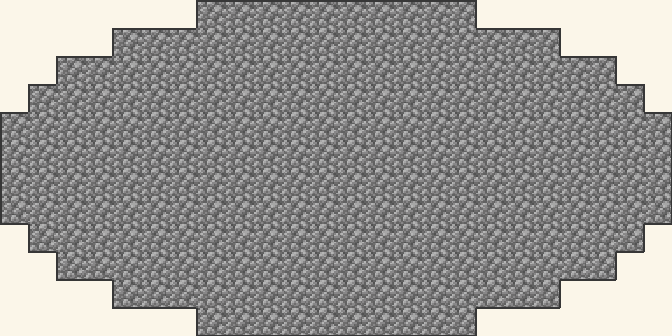
\includegraphics[width=0.45\textwidth]{fig07_2d_ellipse_24x12.png}
\caption{Elipse $W = 24, H = 12$ no Block Round. Note como as celulas ao longo do eixo maior sao mais espacadas que ao longo do eixo menor.}
\label{fig:elipse}
\end{figure}

\begin{enumerate}[leftmargin=1.5em,itemsep=0.15em,topsep=0.3em]
  \item Trocar a forma para \acc{Ellipse}. Aparecem dois \emph{sliders}: \emph{Width} e \emph{Height}.
  \item Definir $W = 24$, $H = 12$. Observar a forma alongada --- ver Figura~\ref{fig:elipse}.
  \item Discutir: \emph{\enquote{A equacao que rege essa forma e $(x/12)^2 + (y/6)^2 = 1$. Por que dividimos $x$ por $12$ e $y$ por $6$?}}
\end{enumerate}

\subsection{Modo 3D, esfera e elipsoide}

\begin{enumerate}[leftmargin=1.5em,itemsep=0.15em,topsep=0.3em]
  \item Trocar o modo para \acc{3D / Sphere}, tamanho $D = 12$.
  \item Arrastar com o \emph{mouse} para rotacionar. Aparece uma esfera composta de voxels.
  \item Acionar o \emph{Info chip}: anotar o volume (\enquote{904 blocks $=14 \times 64 + 8$}).
  \item Trocar para \acc{Ellipsoid}, $W = 20$, $H = 10$, $D = 12$.
  \item Demonstrar o \emph{slider Cut} no eixo \texttt{Y}, 50\% (ver Figura~\ref{fig:cortes}(a)). Observar a metade superior desaparecer.
  \item Alternar para o eixo diagonal $\swarrow$/$\nearrow$ ($45^\circ$, Figura~\ref{fig:cortes}(c)). Discutir o corte obliquo.
\end{enumerate}

\subsection{Exportacao para Minecraft}
\begin{enumerate}[leftmargin=1.5em,itemsep=0.15em,topsep=0.3em]
  \item Mostrar o botao de \emph{download} no canto do canvas: PNG.
  \item Mostrar o botao de \emph{export schematic}: salva um arquivo \texttt{.schem} no formato Sponge v2.
  \item Demonstrar (se possivel) a importacao no Minecraft Java via mod Litematica. Ver Apendice~\ref{ap:litematica}.
\end{enumerate}

% =============================================================================
\newpage
\section{Lista de exercicios}\label{ap:exerc}

\textbf{Instrucoes:} responder individualmente. Pode-se consultar o Block Round para confirmar respostas, \emph{mas a justificativa matematica e obrigatoria}. Entregar manuscrita ou digitada.

\subsection*{Exercicio 1 --- Equacao da circunferencia}
\textbf{Enunciado:} Considere uma circunferencia centrada na origem $(0, 0)$ com raio $r = 7$. Verifique se cada um dos pontos a seguir esta \emph{dentro}, \emph{fora} ou \emph{sobre} a circunferencia. Justifique com a equacao.
\begin{enumerate}[label=\alph*),leftmargin=1.5em,itemsep=0.1em,topsep=0.2em,nosep]
  \item $(3, 4)$ \hfill \emph{gabarito:} dentro ($9 + 16 = 25 < 49$).
  \item $(5, 5)$ \hfill \emph{gabarito:} \acc{fora} ($25 + 25 = 50 > 49$, pois $\sqrt{50} \approx 7{,}07$).
  \item $(0, 7)$ \hfill \emph{gabarito:} sobre.
  \item $(-7, 0)$ \hfill \emph{gabarito:} sobre.
\end{enumerate}

\textit{Atencao pedagogica:} o item (b) e uma armadilha proposital.

\subsection*{Exercicio 2 --- Aritmetica de stacks e baus}
\textbf{Enunciado:} Considere uma esfera $D = 8$ no algoritmo euclidiano, com volume continuo $V = \tfrac{4}{3}\pi \cdot 4^3 \approx 268{,}1$ e volume discreto $V_{\mathrm{disc}} = 268$.
\begin{enumerate}[label=\alph*),leftmargin=1.5em,itemsep=0.1em,topsep=0.2em,nosep]
  \item Quantos stacks de cobblestone sao necessarios para construi-la? Responda na forma $q$ stacks $+$ $r$ blocos extras.
  \item Quantos baus simples (27 slots) sao necessarios para armazenar todos esses stacks?
  \item Em modo survival, supondo coleta de 1 bloco a cada 0{,}5 segundo com pickaxe de ferro, quanto tempo total de coleta?
\end{enumerate}

\emph{Gabarito:} (a) $268 = 4 \times 64 + 12$, ou seja, \acc{4 stacks completos $+$ 12 blocos extras} (5 slots no inventario). (b) 1 bau simples basta (27 slots, ocupam-se apenas 5). (c) $268 \times 0{,}5 = 134$ segundos $\approx$ 2 min 14 s.

\subsection*{Exercicio 3 --- Comparacao de algoritmos para D=20}
\textbf{Enunciado:} No Block Round, gere um circulo de diametro $D = 20$ nos tres algoritmos.
\begin{enumerate}[label=\alph*),leftmargin=1.5em,itemsep=0.1em,topsep=0.2em,nosep]
  \item Anote a area (numero de blocos) de cada algoritmo.
  \item Qual algoritmo minimiza o material? Qual maximiza?
  \item Diferenca em \emph{stacks} entre o maior e o menor? Vale a pena escolher o menor por economia?
\end{enumerate}

\emph{Gabarito esperado:} Euclidiano $\approx 316$ blocos (4 stacks $+$ 60 extra), Bresenham $\approx 316$, Limiar $\approx 332$ blocos (5 stacks $+$ 12 extra). Diferenca: $\approx 1$ stack. Em projeto grande (esferas $D \geq 32$) a economia se acumula.

\subsection*{Exercicio 4 --- Volume de cupula e armazenamento}
\textbf{Enunciado:} Considere uma esfera $D = 16$, algoritmo Euclidiano, cortada em Y a 50\% (cupula classica).
\begin{enumerate}[label=\alph*),leftmargin=1.5em,itemsep=0.1em,topsep=0.2em,nosep]
  \item Volume continuo da esfera completa.
  \item Volume da cupula (metade superior).
  \item Quantos baus duplos sao necessarios para armazenar todos os blocos da cupula?
  \item Sobra material para construir parte do solo (uma camada plana $16 \times 16$ blocos abaixo da cupula)?
\end{enumerate}

\emph{Gabarito:}
(a) $V = \tfrac{4}{3}\pi \cdot 8^3 \approx 2\,144{,}66$, $V_{\mathrm{disc}} \approx 2\,145$. (b) $V_{\mathrm{cupula}} \approx 1\,095$. (c) $\lceil 1\,095 / 3\,456 \rceil = 1$ bau duplo. (d) Sobra: $3\,456 - 1\,095 = 2\,361$ blocos. Solo $16 \times 16 = 256$ blocos. Sobram 2\,105 blocos --- da para construir o solo e mais uma camada de bancada.

\subsection*{Exercicio 5 --- Elipsoide \enquote{mesa redonda gigante}}
\textbf{Enunciado:} Considere um elipsoide com $W = 24$, $H = 8$, $D = 24$ (formato achatado tipo \enquote{mesa}).
\begin{enumerate}[label=\alph*),leftmargin=1.5em,itemsep=0.1em,topsep=0.2em,nosep]
  \item Volume continuo.
  \item Volume discreto estimado no Block Round.
  \item Sobra ou falta material se voce comprou 3 baus duplos de Oak Planks?
\end{enumerate}

\emph{Gabarito:}
(a) $V = \tfrac{4}{3}\pi \cdot 12 \cdot 4 \cdot 12 \approx 2\,413$.
(b) $V_{\mathrm{disc}} \approx 2\,400$ (varia $\pm 10$ por algoritmo).
(c) Capacidade comprada: $3 \times 3\,456 = 10\,368$ blocos. Sobra muito --- $\approx 8\,000$ blocos extras. \emph{Compra exagerada.} O ideal seria 1 bau duplo (sobra de $\approx 1\,000$ blocos).

\subsection*{Exercicio 6 --- WorldEdit vs Block Round}
\textbf{Enunciado:} O comando WorldEdit \cmd{//sphere stone 15} usa um algoritmo similar ao Bresenham 3D. Compare-o com a saida do Block Round no modo Bresenham com $D = 30$:
\begin{enumerate}[label=\alph*),leftmargin=1.5em,itemsep=0.1em,topsep=0.2em,nosep]
  \item Eles devem ser identicos?
  \item Se nao forem, por que? Liste pelo menos dois motivos.
\end{enumerate}

\emph{Gabarito:}
(a) \emph{Aproximadamente sim} --- ambos sao Bresenham 3D, mas (b) podem diferir por: (i) implementacoes diferentes (Block Round e em JavaScript; WorldEdit e em Java); (ii) tratamento da paridade do diametro (par vs impar); (iii) constante empirica de \emph{threshold} (se algum dos dois usa Limiar internamente). Tipica diferenca: 0--6 blocos para $D = 30$.

\subsection*{Exercicio 7 --- Construcao por simetria octaedrica}
\textbf{Enunciado:} Projetar a construcao de uma esfera $D = 16$ centrada em $(0, 72, 0)$ no Minecraft, usando simetria. Construir 1 octante (regiao $+x, +y, +z$, $\approx 268$ blocos) e refletir 7 vezes via \cmd{/clone}.
\begin{enumerate}[label=\alph*),leftmargin=1.5em,itemsep=0.1em,topsep=0.2em,nosep]
  \item Escreva os 7 comandos \cmd{/clone} (use \cmd{mode:masked} para nao apagar terreno).
  \item Calcule o tempo total estimado: construcao manual do octante + comandos.
\end{enumerate}

\emph{Gabarito:}

\begin{minec}[Sequencia de comandos]
\cmd{/clone 0 72 0 7 79 7 -8 72 0 mode:masked} \quad (reflex.\ $-x$)\\
\cmd{/clone 0 72 0 7 79 7 0 64 0 mode:masked} \quad\quad (reflex.\ $-y$)\\
\cmd{/clone 0 72 0 7 79 7 0 72 -8 mode:masked} \quad (reflex.\ $-z$)\\
\cmd{/clone -8 72 0 -1 79 7 mode:masked} \quad\quad\;\; (octante $-x,-y$)\\
\cmd{/clone 0 64 -8 7 71 -1 mode:masked} \quad\quad\;\; (octante $-y,-z$)\\
\cmd{/clone -8 72 -8 -1 79 -1 mode:masked} \quad\;\; (octante $-x,-z$)\\
\cmd{/clone -8 64 -8 -1 71 -1 mode:masked} \quad\;\; (octante $-x,-y,-z$)
\end{minec}

Tempo: $\sim$\,5 min (octante manual em survival) + $\sim$\,3 s (7 clones).

\subsection*{Exercicio 8 --- Projeto final}
\textbf{Enunciado:} Apos produzir a construcao em grupo (Atividade~\ref{at:53}), responda:
\begin{enumerate}[label=(\arabic*),leftmargin=1.7em,itemsep=0.15em,topsep=0.2em,nosep]
  \item Liste as figuras geometricas usadas (circulo, elipse, esfera, elipsoide) e seus parametros (diametro ou semi-eixos).
  \item Para a figura principal, qual algoritmo foi escolhido? Por que? Que efeito visual ele produz que os outros dois nao produziriam?
  \item Houve cortes 3D? Se sim, descreva matematicamente \emph{um} deles como desigualdade.
  \item Quantos stacks/baus seriam necessarios para construir realmente no Minecraft em survival?
  \item Sua producao dialoga com alguma referencia cultural brasileira (modernismo, arte concreta, grafismo indigena, arquitetura de Niemeyer, comunidade Minecraft BR)? Comente.
\end{enumerate}

% =============================================================================
\newpage
\section{Adaptacao para escolas sem laboratorio de informatica}\label{ap:adapt-analog}

Esta adaptacao possibilita aplicar a sequencia \emph{integralmente em papel} quando o acesso a computador estiver inviabilizado --- realidade frequente em escolas do campo, escolas indigenas e quilombolas, em comunidades ribeirinhas da Amazonia, e em escolas estaduais de pequenos municipios. O eixo conceitual permanece intacto; o que muda e o suporte material.

\subsection{Substituicoes por aula}

\begin{center}
\small
\begin{tabularx}{\textwidth}{@{}p{0.13\textwidth}p{0.32\textwidth}X@{}}
\toprule
\textbf{Aula} & \textbf{Atividade original} & \textbf{Adaptacao analogica} \\
\midrule
1 & Demonstracao do Block Round (1.3) & Professor desenha a mao tres versoes da circunferencia $D = 10$ em uma malha pre-impressa do tamanho da lousa --- uma por algoritmo. As Figuras~\ref{fig:comp-d10} e~\ref{fig:comp-d20} podem ser impressas como referencia. \\
\addlinespace[3pt]
2 & Comparacao quantitativa no software (\ref{at:25}) & Distribuir folhas com as tres circunferencias de $D = 16$ pre-desenhadas e pedir a contagem manual. \\
\addlinespace[3pt]
3 & Geracao da esfera 3D (\ref{at:31},~\ref{at:32}) & Distribuir folhas com \emph{fatias} da esfera ($z = 0, 1, 2, \ldots$) em papel quadriculado. O estudante constroi o modelo mental por empilhamento. Cada folha simula uma \emph{camada} de blocos do Minecraft. \\
\addlinespace[3pt]
4 & Comandos Minecraft (\ref{at:42}) & Substituir comandos por \emph{instrucoes de construcao} escritas em portugues; estudantes simulam a execucao em papel quadriculado. \\
\addlinespace[3pt]
5 & Construcao real em Minecraft (\ref{at:53}) & Construcao em \emph{LEGO} (se disponivel), em papel quadriculado colorido com lapis verde-grama e marrom-terra, ou em \emph{cubos de papel} dobrados pelos estudantes em aula de Arte. \\
\bottomrule
\end{tabularx}
\end{center}

\subsection{Folhas auxiliares}
Para a versao analogica completa, recomenda-se preparar previamente:
\begin{itemize}[leftmargin=1.3em,itemsep=0.1em,topsep=0.2em,nosep]
  \item 1 folha A3 com malha $30 \times 30$ desenhada com regua.
  \item 1 conjunto por estudante de 5 folhas A4 quadriculadas (5\,mm).
  \item 1 folha com as tres circunferencias comparativas pre-impressas: as Figuras~\ref{fig:comp-d10} e~\ref{fig:comp-d20} deste plano, em A4, servem como referencia.
  \item Para a Aula 5 analogica: 8 cubos de papel pre-dobrados por grupo (representando blocos de cobblestone, oak, quartz, diamond).
\end{itemize}

\subsection{Aproveitamento de saberes locais}
Em escolas indigenas ou em comunidades com forte tradicao artesanal (renda de bilro em Aracati/CE, ceramica em Pirenopolis/GO, tecelagem caicara no litoral norte de SP, ceramica marajoara no Para, cestaria Pankararu de PE), a Aula~\ref{aula3} pode ser \emph{enriquecida com uma visita de portadores de saber tradicional}: rendeiras, tecelas, ceramistas, mostrando como rasterizam circulos em suas linguagens proprias. Essa aproximacao realiza o principio etnomatematico e a \href{https://www.planalto.gov.br/ccivil_03/_ato2007-2010/2008/lei/l11645.htm}{Lei 11.645/2008}.

% =============================================================================
\newpage
\section{Glossario tecnico para o professor}\label{ap:glos}

\begin{itemize}[leftmargin=1.4em,itemsep=0.3em,topsep=0.3em]
  \item \acc{Algoritmo} --- sequencia finita e bem definida de instrucoes para resolver um problema. Os tres algoritmos do Block Round (cf.\ Figura~\ref{fig:comp-d10}) sao procedimentos distintos para o mesmo problema.
  \item \acc{Bau (simples)} --- container do Minecraft com 27 slots. Capacidade: $27 \times 64 = 1\,728$ itens.
  \item \acc{Bau duplo} --- dois baus adjacentes que se combinam em um container de 54 slots. Capacidade: $54 \times 64 = 3\,456$ itens.
  \item \acc{Bloco} --- unidade construtiva de Minecraft. Cubo $1\times1\times1$ com seis faces texturizadas. Em linguagem matematica, e um \emph{voxel}.
  \item \acc{Bresenham (algoritmo de)} --- algoritmo publicado em 1965 por Jack Bresenham (IBM), originalmente para reta, depois estendido por outros autores (Pitteway, Kappel) para elipse. Sua marca e usar \emph{apenas inteiros}. Veja Atividade~\ref{at:23}.
  \item \acc{BNCC} --- Base Nacional Comum Curricular. Documento normativo brasileiro de referencia para a Educacao Basica, aprovado em 2017 (EI/EF) e 2018 (EM).
  \item \acc{Canvas} --- elemento HTML que disponibiliza um espaco de desenho 2D ou 3D no navegador.
  \item \acc{\code{/clone}} --- comando vanilla do Minecraft que copia uma regiao retangular para outra posicao. Sintaxe: \cmd{/clone x1 y1 z1 x2 y2 z2 dx dy dz}. Essencial para construcao por simetria.
  \item \acc{ENEM} --- Exame Nacional do Ensino Medio.
  \item \acc{Equacao implicita} --- equacao da forma $F(x, y) = 0$. A da elipse: $(x/r_x)^2 + (y/r_y)^2 - 1 = 0$.
  \item \acc{Etnomatematica} --- campo de estudos fundado pelo brasileiro Ubiratan D'Ambrosio.
  \item \acc{\code{/fill}} --- comando vanilla do Minecraft que preenche uma caixa retangular com um tipo de bloco. Sintaxe: \cmd{/fill x1 y1 z1 x2 y2 z2 minecraft:stone}.
  \item \acc{IMPA} --- Instituto de Matematica Pura e Aplicada (\url{https://impa.br}). Centro de pesquisa de referencia mundial sediado no Rio de Janeiro. Organizador da \hyperref[sec:obmep]{OBMEP}.
  \item \acc{LGPD} --- Lei Geral de Protecao de Dados Pessoais (Lei 13.709/2018).
  \item \acc{Litematica} --- mod popular do Minecraft Java Edition que importa schematics e mostra um \emph{fantasma} translucido da construcao a ser realizada bloco a bloco. Gratuito.
  \item \acc{Minecraft Education Edition} --- versao educacional do Minecraft, gratuita para escolas via parceria MEC--Microsoft.
  \item \acc{OBMEP} --- Olimpiada Brasileira de Matematica das Escolas Publicas.
  \item \acc{Pack / Stack} --- pilha de ate 64 blocos identicos em um slot do inventario do Minecraft.
  \item \acc{Pixel} --- abreviacao de \emph{picture element}. Em 2D.
  \item \acc{PWA} --- \emph{Progressive Web App}. Aplicacao \emph{web} instalavel e operavel \emph{offline}.
  \item \acc{Rasterizacao} --- processo de converter uma descricao geometrica continua em uma matriz de pixels (2D) ou voxels (3D).
  \item \acc{Schematica} --- mod alternativo a Litematica, com funcao semelhante.
  \item \acc{Schematic (\texttt{.schem})} --- formato de arquivo que serializa uma regiao do Minecraft (Sponge Schematic v2, gzip + NBT).
  \item \acc{Semi-eixo} --- em uma elipse, distancia do centro a extremidade na direcao do eixo.
  \item \acc{\code{//sphere}} --- comando WorldEdit que constroi uma esfera. Sintaxe: \cmd{//sphere bloco raio}.
  \item \acc{Slot} --- celula individual no inventario do Minecraft. Inventario completo do jogador: 36 slots ($9 \times 4$).
  \item \acc{Voxel} --- abreviacao de \emph{volume element}. Generalizacao do pixel para 3D. Em Minecraft, cada \emph{bloco} e um voxel.
  \item \acc{WebGL} --- biblioteca de programacao grafica em 3D para navegadores.
  \item \acc{WorldEdit} --- mod muito popular do Minecraft Java que adiciona comandos avancados de construcao em larga escala, incluindo \cmd{//sphere}, \cmd{//hsphere}, \cmd{//ellipsoid}, \cmd{//cyl}, \cmd{//schem load}.
\end{itemize}

% =============================================================================
\newpage
\section{Tutorial: do Block Round ao Minecraft via Litematica}\label{ap:litematica}

Este apendice descreve o fluxo completo de exportacao do Block Round e importacao no Minecraft Java Edition usando o mod \emph{Litematica}. Tempo total esperado: 15 minutos (primeira vez).

\subsection{Pre-requisitos}
\begin{itemize}[leftmargin=1.3em,itemsep=0.1em,topsep=0.2em,nosep]
  \item Minecraft Java Edition (compra na \emph{Mojang Store}; versao educacional gratuita \emph{Minecraft Education} tambem funciona, com ajustes).
  \item \emph{Fabric Loader} para a versao do Minecraft que voce usa (geralmente a mais recente: \url{https://fabricmc.net/use/}).
  \item Mods: \emph{Fabric API} e \emph{Litematica} (\url{https://www.curseforge.com/minecraft/mc-mods/litematica}).
  \item Block Round aberto no navegador, com a figura desejada ja produzida.
\end{itemize}

\subsection{Passo 1: exportar do Block Round}
\begin{enumerate}[leftmargin=1.5em,itemsep=0.15em,topsep=0.3em]
  \item No Block Round, configure a figura desejada (modo, forma, diametro, algoritmo, bloco, corte). Verifique no \emph{Info chip} o volume.
  \item Clique no botao \emph{Export Schematic} (canto superior direito do canvas, segundo icone). Um arquivo \texttt{.schem} sera baixado.
\end{enumerate}

\subsection{Passo 2: instalar Litematica}
\begin{enumerate}[leftmargin=1.5em,itemsep=0.15em,topsep=0.3em]
  \item Instale o Fabric Loader na versao do Minecraft que voce usa.
  \item Baixe \emph{Fabric API} e \emph{Litematica} para a mesma versao do Minecraft. Coloque ambos no diretorio \texttt{.minecraft/mods/}.
  \item Inicie o Minecraft com o perfil \emph{fabric-loader-x.y.z-1.20.x}.
\end{enumerate}

\subsection{Passo 3: importar o schematic}
\begin{enumerate}[leftmargin=1.5em,itemsep=0.15em,topsep=0.3em]
  \item Coloque o arquivo \texttt{.schem} em \texttt{.minecraft/schematics/} (ou na pasta padrao do Litematica, definida nas Configuracoes do mod).
  \item Em um mundo (criativo ou sobrevivencia), aperte \texttt{M} para abrir o menu da Litematica.
  \item Clique em \emph{Load Schematic} $\rightarrow$ selecione o arquivo $\rightarrow$ \emph{Load}.
  \item O schematic agora aparece em uma lista. Clique nele e em \emph{Placement}: o \enquote{fantasma} translucido da figura aparece no mundo.
  \item Use os controles de movimento (\texttt{M} $\rightarrow$ \emph{Placements}) para arrastar o fantasma para a posicao desejada. Para terreno plano, basta posicionar o canto inferior $(x_1, y_1, z_1)$ no chao.
\end{enumerate}

\subsection{Passo 4: construir}
\begin{enumerate}[leftmargin=1.5em,itemsep=0.15em,topsep=0.3em]
  \item Em \emph{Creative}: voe sobre o fantasma e coloque cada bloco onde a Litematica mostra; o mod confirma com verde os blocos corretos e marca em vermelho qualquer erro. A construcao de uma esfera $D = 12$ leva $\approx$\,5 minutos.
  \item Em \emph{Survival}: identico, mas voce precisa coletar os blocos antes. Use o calculo de stacks/baus da Atividade~\ref{at:41} para planejar a coleta.
  \item Alternativa: se o servidor tem WorldEdit, use \cmd{//schem load nome-arquivo} seguido de \cmd{//paste -a} para construcao instantanea.
\end{enumerate}

\subsection{Passo 5: verificacao}
A Litematica destaca em vermelho qualquer bloco que esteja errado (faltando, do tipo errado, ou em posicao errada). Use o atalho \texttt{Z} para alternar entre \emph{visivel} e \emph{invisivel} o fantasma, comparando com a construcao real.

\subsection{Solucao de problemas comuns}
\begin{itemize}[leftmargin=1.3em,itemsep=0.15em,topsep=0.3em,nosep]
  \item \emph{Schematic nao aparece na lista:} verifique se o arquivo esta na pasta certa, e se a versao da Litematica e compativel com a do Minecraft.
  \item \emph{Blocos errados/aparecem cinza:} alguns blocos no schematic do Block Round podem nao estar disponiveis no mundo (versao antiga do Minecraft); abra o schematic com texteditor para conferir nomes.
  \item \emph{Fantasma flutua:} ajuste a posicao com a opcao \emph{Rotation/Mirror} no menu de Placement. Para esferas, e indiferente; para elipses, ajuste a rotacao.
\end{itemize}

\vspace{2em}
\begin{center}
\color{muted}\small\sffamily
--- fim do plano de aula ---
\end{center}

\end{document}
